% STATUS: ACTIVE | DERIVATION (2026-09-20) of the offset law: the exact plane polynomial evaluated at the distance to an
%   EFFECTIVE wall, delta = depth of the hydrodynamic (no-slip) wall below the known reference surface w_s, in R. One
%   position-type state, zero shape constants (ledger C62: cell = plane slid down 1.05 R; C53: position-type unknowns
%   belong in a position container). Written for the two places the unknown can live, as in 0916_estb_11_two_versions.tex:
%   A -- delta as a constant state with the gain COMPUTED from the law at the estimator's own height (no a slot);
%   B -- an a slot carried along the AUTONOMOUS form of the law, which is delta-free, so delta enters B only through the seed.
%   Coordinate: h = w - w_s (centre height above the reference surface; plane: the wall, contact at 1; cell: the visible
%   surface), g = h + delta = centre distance to the effective wall (contact of the polynomial at g = 1).
%   Same nine-section reading copy; paper observability gates 1-3 for delta (observability-workflow.md) in the
%   Observability section; the numerical gates run verify_state_observability.m. Independent check of every closed form:
%   test_script/scratch/check_estb_delta_jacobians.py (sympy). Related: Meng dissertation 6.2 inverts the same C_perp
%   from an already-estimated gain in a separate 1-state EKF (ledger C63); here the inversion is the y_2 row of one filter.
%   Plant of the tests: plane = calc_correction_functions; cell = test_script/scratch/cell_cperp_delta.m (delta = 1.05).
% Compile: xelatex 0920_estb_delta_law.tex

\documentclass[11pt,a4paper,fontset=none]{ctexart}
\usepackage[fleqn]{amsmath}
\usepackage{amssymb,bm}
\setlength{\mathindent}{0pt}
\usepackage{graphicx}
\usepackage{pdflscape}
\usepackage{geometry}
\geometry{margin=2.0cm}

\setlength{\parindent}{0pt}
\setlength{\parskip}{0.80em}
\linespread{1.08}
\setlength{\abovedisplayskip}{10pt}
\setlength{\belowdisplayskip}{10pt}

\newcommand{\ba}{\bar{a}}
\newcommand{\bw}{\bar{w}}
\newcommand{\dW}{\Delta\bw}
\newcommand{\ap}{\ba'}
\newcommand{\app}{\ba''}
\newcommand{\ah}{\hat{\ba}_w}
\newcommand{\wh}{\hat{\bw}}
\newcommand{\ad}{\hat{\ba}_d}
\newcommand{\Dp}{D_{\perp}}
\newcommand{\dl}{\delta}
\newcommand{\dlh}{\hat{\delta}}
\newcommand{\gh}{\hat{g}}
\newcommand{\lam}{\Lambda}

\begin{document}

\section{Gain law}

(bars denote normalized quantities: lengths by $R$; $a_o := \Delta t/(\gamma_N R)$ [1/pN]; $\ba := a/a_{\mathrm{nom}}$;
$\bar f := a_o f$, so that $\ba\,\bar f = \dW$; $\bw$ = particle centre along the wall normal; $\bw_s$ = the known reference
surface on the same axis (plane: the wall, so $\bw - \bw_s = \bar h$ with contact at 1; cell: the visible surface);
$\dl$ = depth of the effective (hydrodynamic) wall below $\bw_s$, in $R$, the one constant of the wall;
$g := (\bw - \bw_s) + \dl$ = centre distance to the effective wall, the law is used on $g \ge 1.1$;
$u := 1/g$; $e_\theta = \theta - \hat\theta$)

\begin{align*}
\Dp(u)                 &= 1 - \tfrac{9}{8}u + \tfrac{1}{2}u^{3} - \tfrac{57}{100}u^{4} + \tfrac{1}{5}u^{5} + \tfrac{7}{200}u^{11} - \tfrac{1}{25}u^{12} \\[4pt]
\ba(\bw;\,\dl)         &= \Dp\!\Bigl(\frac{1}{(\bw - \bw_s) + \dl}\Bigr) \\[4pt]
\ap(\bw;\,\dl)         &:= \frac{\partial\ba}{\partial\bw} = -\,u^{2}\,\Dp'(u) \\[4pt]
\app(\bw;\,\dl)        &:= \frac{\partial^{2}\ba}{\partial\bw^{2}} = u^{4}\,\Dp''(u) + 2u^{3}\,\Dp'(u) \\[4pt]
\Bigl(\frac{\partial\ba}{\partial\dl}\Bigr)_{\bw}   &= \ap, \qquad
\Bigl(\frac{\partial\ba}{\partial\bw_s}\Bigr)_{\bw} = -\,\ap, \qquad
\frac{\partial\ap}{\partial\dl} = \app \\[4pt]
\Dp(1) &= 0, \qquad -\,\Dp'(1) = 1, \qquad \lim_{u\to 0}\frac{1-\Dp(u)}{u} = \tfrac{9}{8} \\[4pt]
\ap &= \lam(\ba) := -\,u(\ba)^{2}\,\Dp'\bigl(u(\ba)\bigr), \qquad u(\ba) := \Dp^{-1}(\ba)\ \text{on } u \in (0, 1], \qquad
\frac{\partial\lam}{\partial\dl} = 0 \\[4pt]
\frac{d\lam}{d\ba} &= \frac{\app}{\ap} \\[4pt]
a_w &= a_o\,\ba_w
\end{align*}

\section{True dynamics}

$\bigl(\delta\bw_j[k] := \delta\bw[k-d+j-1],\ j = 1,\dots,d+1,\ d = 2\bigr)$

\begin{align*}
\bw[k]           &= \bw_d[k] - \delta\bw_3[k] \\
\bw_d[k+1]       &= \bw_d[k] + \Delta\bw_d[k] \\
\ba_w[k]         &= \Dp\!\Bigl(\frac{1}{(\bw[k] - \bw_s) + \dl}\Bigr) \\
\delta\bw_1[k+1] &= \delta\bw_2[k] \\
\delta\bw_2[k+1] &= \delta\bw_3[k] \\
\delta\bw_3[k+1] &= \lambda_c\,\delta\bw_3[k] - F_{dw}[k]\,e_{\ba_w}[k] - \varepsilon_w[k] \\
\dW[k]           &= \Delta\bw_d[k] + (1-\lambda_c)\,\delta\bw_3[k] + F_{dw}[k]\,e_{\ba_w}[k] + \varepsilon_w[k] \\
\dl[k+1]         &= \dl[k]
\end{align*}

\begin{align*}
F_{dw}[k]        &= \bar f_{dw}[k] + (1-\lambda_c)\sum_{i=1}^{d}\bar f_{dw}[k-i] \\
\varepsilon_w[k] &= \ba_w[k]\,\bar f_T[k] + (1-\lambda_c)\sum_{i=1}^{d}\ba_w[k-i]\,\bar f_T[k-i] - (1-\lambda_c)\,n_w[k]
\end{align*}

\section{Estimator A: $\dl$ as a state, gain computed (no $a$ slot)}

\begin{align*}
\mathbf{x}_A &= \bigl[\,\delta\bw_1,\ \delta\bw_2,\ \delta\bw_3,\ \dl\,\bigr]^{\top}
\end{align*}

\begin{align*}
\wh[k]                 &= \bw_d[k] - \delta\hat{\bw}_3[k] \\
\gh[k]                 &= (\wh[k] - \bw_s) + \dlh[k] \\
\ah[k]                 &= \Dp\!\Bigl(\frac{1}{\gh[k]}\Bigr) \\
\delta\hat{\bw}_1[k+1] &= \delta\hat{\bw}_2[k] \\
\delta\hat{\bw}_2[k+1] &= \delta\hat{\bw}_3[k] \\
\delta\hat{\bw}_3[k+1] &= \lambda_c\,\delta\hat{\bw}_3[k] \\
\dlh[k+1]              &= \dlh[k]
\end{align*}

\section{Error dynamics A}

$\bigl(\mathbf{e}_A = [\,e_{\delta\bw_1},\ e_{\delta\bw_2},\ e_{\delta\bw_3},\ e_{\dl}\,]^{\top}$; coefficients at the estimate, $\ap[k] := \ap(\gh[k])\bigr)$

\begin{align*}
e_{\ba_w}[k]         &= \ap[k]\,\bigl(e_{\dl}[k] - e_{\delta\bw_3}[k]\bigr) \\[6pt]
e_{\delta\bw_1}[k+1] &= e_{\delta\bw_2}[k] \\
e_{\delta\bw_2}[k+1] &= e_{\delta\bw_3}[k] \\
e_{\delta\bw_3}[k+1] &= \bigl(\lambda_c + F_{dw}[k]\,\ap[k]\bigr)\,e_{\delta\bw_3}[k] - F_{dw}[k]\,\ap[k]\,e_{\dl}[k] - \varepsilon_w[k] \\
e_{\dl}[k+1]         &= e_{\dl}[k]
\end{align*}

\begin{align*}
F_e^{A}[k] &= \begin{bmatrix}
0 & 1 & 0 & 0 \\
0 & 0 & 1 & 0 \\
0 & 0 & \lambda_c + F_{dw}[k]\,\ap[k] & -F_{dw}[k]\,\ap[k] \\
0 & 0 & 0 & 1
\end{bmatrix}
\end{align*}

\begin{align*}
\mathrm{Var}\bigl(e_{\ba_w}[k]\bigr) &= \ap[k]^{2}\,\bigl(P_{33}[k] + P_{44}[k] - 2P_{34}[k]\bigr)
\end{align*}

\section{Estimator B: $a$ slot carried along the autonomous law (no $\dl$ state)}

$\bigl(M[k] := \Delta\bw_d[k] + (1-\lambda_c)\,\delta\hat{\bw}_3[k]$; $\lam$ does not contain $\dl$, so $\dl$ has no column in any row of B and enters only through $\ah[0]$ and $P_{44}[0]\bigr)$

\begin{align*}
\mathbf{x}_B &= \bigl[\,\delta\bw_1,\ \delta\bw_2,\ \delta\bw_3,\ \ba_w\,\bigr]^{\top}
\end{align*}

\begin{align*}
\delta\hat{\bw}_1[k+1] &= \delta\hat{\bw}_2[k] \\
\delta\hat{\bw}_2[k+1] &= \delta\hat{\bw}_3[k] \\
\delta\hat{\bw}_3[k+1] &= \lambda_c\,\delta\hat{\bw}_3[k] \\
\ah[k+1]               &= \Dp\!\Bigl(\frac{1}{\,1/u(\ah[k]) + M[k]\,}\Bigr) \\
                       &= \ah[k] + \lam\bigl(\ah[k]\bigr)\,M[k] + \tfrac{1}{2}\,\app\bigl(\ah[k]\bigr)\,M[k]^{2} + \dots
\end{align*}

\section{Error dynamics B}

$\bigl(\mathbf{e}_B = [\,e_{\delta\bw_1},\ e_{\delta\bw_2},\ e_{\delta\bw_3},\ e_{\ba_w}\,]^{\top}$; first-order step, coefficients at the estimate$\bigr)$

\begin{align*}
e_{\delta\bw_1}[k+1] &= e_{\delta\bw_2}[k] \\
e_{\delta\bw_2}[k+1] &= e_{\delta\bw_3}[k] \\
e_{\delta\bw_3}[k+1] &= \lambda_c\,e_{\delta\bw_3}[k] - F_{dw}[k]\,e_{\ba_w}[k] - \varepsilon_w[k] \\
e_{\ba_w}[k+1]       &= (1-\lambda_c)\,\lam\bigl(\ah[k]\bigr)\,e_{\delta\bw_3}[k]
                        + \Bigl(1 + \lam\bigl(\ah[k]\bigr)\,F_{dw}[k] + \frac{\app(\ah[k])}{\ap(\ah[k])}\,M[k]\Bigr)e_{\ba_w}[k] \\
                     &\quad + \lam\bigl(\ah[k]\bigr)\,\varepsilon_w[k]
\end{align*}

\begin{align*}
F_e^{B}[k] &= \begin{bmatrix}
0 & 1 & 0 & 0 \\
0 & 0 & 1 & 0 \\
0 & 0 & \lambda_c & -F_{dw}[k] \\
0 & 0 & (1-\lambda_c)\,\lam(\ah[k]) & 1 + \lam(\ah[k])\,F_{dw}[k] + \dfrac{\app(\ah[k])}{\ap(\ah[k])}\,M[k]
\end{bmatrix}
\end{align*}

\section{Measurement}

$\bigl(\nabla_d\bw_d[k] := \bw_d[k] - \bw_d[k-d]$; $\wh_d[k] := \wh[k] - \nabla_d\bw_d[k]$; $\gh_d[k] := (\wh_d[k] - \bw_s) + \dlh[k]\bigr)$

\begin{align*}
y_1[k]      &= \delta\bw_1[k] + n_w[k] \\
y_2[k]      &= \ba_w[k-d] + n_a[k] \\
\hat y_1[k] &= \delta\hat{\bw}_1[k]
\end{align*}

\begin{align*}
\text{A:}\qquad
\ad[k]      &= \Dp\!\Bigl(\frac{1}{\gh_d[k]}\Bigr) \\
\hat y_2[k] &= \ad[k] \\
H^{A}[k]    &= \begin{bmatrix} 1 & 0 & 0 & 0 \\
               0 & 0 & -\,\ap(\gh_d[k]) & \ap(\gh_d[k]) \end{bmatrix}
\end{align*}

\begin{align*}
\text{B:}\qquad
\ad[k]      &= \Dp\!\Bigl(\frac{1}{\,1/u(\ah[k]) - \nabla_d\bw_d[k]\,}\Bigr) \\
\hat y_2[k] &= \ad[k] \\
\frac{\partial\ad[k]}{\partial\ah[k]} &= \frac{\lam(\ad[k])}{\lam(\ah[k])} \\
H^{B}[k]    &= \begin{bmatrix} 1 & 0 & 0 & 0 \\
               0 & 0 & 0 & \dfrac{\lam(\ad[k])}{\lam(\ah[k])} \end{bmatrix}
\end{align*}

\begin{align*}
\mathbf{e}_y[k] &= H[k]\,\mathbf{e}^{-}[k] + \begin{bmatrix} n_w[k] \\ n_a[k] \end{bmatrix}
\end{align*}

\section{Noise}

\begin{align*}
Q^{A}[k]  &= Q_{33}[k]\,\mathbf{g}_A\,\mathbf{g}_A^{\top}, \qquad \mathbf{g}_A = \bigl[\,0,\ 0,\ -1,\ 0\,\bigr]^{\top} \\
Q^{B}[k]  &= Q_{33}[k]\,\mathbf{g}_B\,\mathbf{g}_B^{\top}, \qquad
\mathbf{g}_B = \bigl[\,0,\ 0,\ -1,\ \lam(\ah[k])\,\bigr]^{\top} \\
Q_{33}[k] &= \kappa_T\Bigl(\ah[k] + (1-\lambda_c)^{2}\bigl(\ah[k-1] + \ah[k-2]\bigr)\Bigr) + (1-\lambda_c)^{2}\sigma^{2}_{n_w},
\qquad \kappa_T = \frac{4k_BT\,a_o}{R} \\
R[k]      &= \mathrm{diag}\bigl(R_1,\ R_2[k]\bigr), \qquad R_1 = \frac{\sigma^{2}_{n}}{R^{2}}, \qquad
R_2[k] = 2a_{\mathrm{cov}}^{2}\,IF_{\mathrm{var}}\bigl(\ah[k]\bigr)\bigl(\ah[k] + \xi\bigr)^{2}
\end{align*}

\clearpage
\section{Observability}

($\Phi(k,k_0) := F_e[k-1]\cdots F_e[k_0]$, $\Phi(k_0,k_0) = I$; $N$ window length)

($O_w := R_w^{-1/2}\,[\,H[k_0]\Phi(k_0,k_0);\ \dots;\ H[k_0+N]\Phi(k_0+N,k_0)\,]$;
$O_w\,\mathbf{v}_i = \sigma_i\,\mathbf{u}_i$; $\sigma_\theta := \sqrt{[(O_w^{\top}O_w)^{-1}]_{\theta\theta}}$)

Gate 1, the two columns of $e_{\dl}$ (A):
\begin{align*}
F^{A}_{e,34}[k] &= -\,F_{dw}[k]\,\ap(\gh[k]), \qquad H^{A}_{24}[k] = \ap(\gh_d[k])
\end{align*}

Gate 2, time signatures of the pair $(e_{\delta\bw_3},\ e_{\dl})$ (A):
\begin{align*}
e_{\dl}[k+1]         &= e_{\dl}[k] \\
e_{\delta\bw_3}[k+1] &= \bigl(\lambda_c + F_{dw}[k]\,\ap[k]\bigr)\,e_{\delta\bw_3}[k] - F_{dw}[k]\,\ap[k]\,e_{\dl}[k] - \varepsilon_w[k], \qquad
y_1[k+2] = e_{\delta\bw_3}[k] + \dots
\end{align*}

Gate 3, $\det O_2$ of the pair with coefficients frozen ($\alpha := \lambda_c + F_{dw}\,\ap(\gh)$, $\beta := F_{dw}\,\ap(\gh)$, $p := \ap(\gh_d)$):
\begin{align*}
A_2 &= \begin{bmatrix} \alpha & -\beta \\ 0 & 1 \end{bmatrix} \\[4pt]
\text{row } y_1 \text{ only:}\quad C_2 &= \bigl[\,1,\ 0\,\bigr], \qquad
\det\begin{bmatrix} C_2 \\ C_2A_2 \end{bmatrix} = -\,\beta = -\,F_{dw}\,\ap(\gh) \\[4pt]
\text{row } y_2 \text{ only:}\quad C_2 &= \bigl[\,-p,\ p\,\bigr], \qquad
\det\begin{bmatrix} C_2 \\ C_2A_2 \end{bmatrix} = p^{2}\,(\alpha - \beta - 1) = -\,(1-\lambda_c)\,\ap(\gh_d)^{2}
\end{align*}

\begin{align*}
\det O_2 = 0 \ (y_1) \quad&\Longleftrightarrow\quad F_{dw} = 0 \ \text{(hold)} \ \ \text{or}\ \ \ap(\gh) = 0 \ \text{(far field)} \\
\det O_2 = 0 \ (y_2) \quad&\Longleftrightarrow\quad \ap(\gh_d) = 0 \ \text{(far field only)}
\end{align*}

Aliases (A):
\begin{align*}
\Bigl(\frac{\partial\ba}{\partial\dl}\Bigr)_{\bw} + \Bigl(\frac{\partial\ba}{\partial\bw_s}\Bigr)_{\bw} &= 0
\quad\Longrightarrow\quad \text{only } \bw_s - \dl \text{ enters; } \bw_s \text{ is given, not a state} \\
\ap(\gh) \to 0 \ \text{(far field)} \quad&\Longrightarrow\quad F^{A}_{e,34} \to 0,\ H^{A}_{24} \to 0,\ e_{\dl} \ \text{unobservable}
\end{align*}

B:
\begin{align*}
\frac{\partial\lam}{\partial\dl} = 0,\quad \frac{\partial H^{B}}{\partial\dl} = 0,\quad \frac{\partial F_e^{B}}{\partial\dl} &= 0 \\
&\Longrightarrow\quad \dl \ \text{has no column in any row of B} \\
&\Longrightarrow\quad \text{gate 1 fails by construction: } \dl \ \text{is not a state of B}
\end{align*}

\section*{Seed and prior}

\begin{align*}
&\text{plant offsets:}\quad \dl_{\mathrm{plane}} = 0, \qquad \dl_{\mathrm{cell}} = 1.05 \ \ (\texttt{cell\_cperp\_delta}) \\
&\text{wall family prior (half the plane--cell spread, two-sided):}\quad \sigma_{\dl,0} = 0.5 \\[4pt]
\text{arm T:}\quad \dlh[0] &= \dl_{\mathrm{plant}} \\
\text{arm T}\pm\text{:}\quad \dlh[0] &= \dl_{\mathrm{plant}} \pm 0.5 \\
\text{arm W:}\quad \bw_s &\to \bw_s + 1, \qquad \dlh[0] = \dl_{\mathrm{plant}} \\
\ah[0] &= \Dp\!\Bigl(\frac{1}{(\bw[0] - \bw_s) + \dlh[0]}\Bigr) \\
P[0]   &= \mathrm{diag}\bigl(P_{11}[0],\ P_{22}[0],\ P_{33}[0],\ P_{44}[0]\bigr) \\
\text{A:}\quad \sqrt{P_{44}[0]} &= \sigma_{\dl,0}, \qquad Q_{44} = 0 \\
\text{B:}\quad P_{44}[0] &= \ap\bigl(\gh[0]\bigr)^{2}\,\sigma_{\dl,0}^{2} \\[4pt]
\text{guard:}\quad \gh[k] &\ge 1 \quad(\text{the polynomial is evaluated at } \max(\gh[k],\ 1)), \qquad \text{band } \gh \ge 1.1
\end{align*}

\begin{landscape}
\vspace*{\fill}
\noindent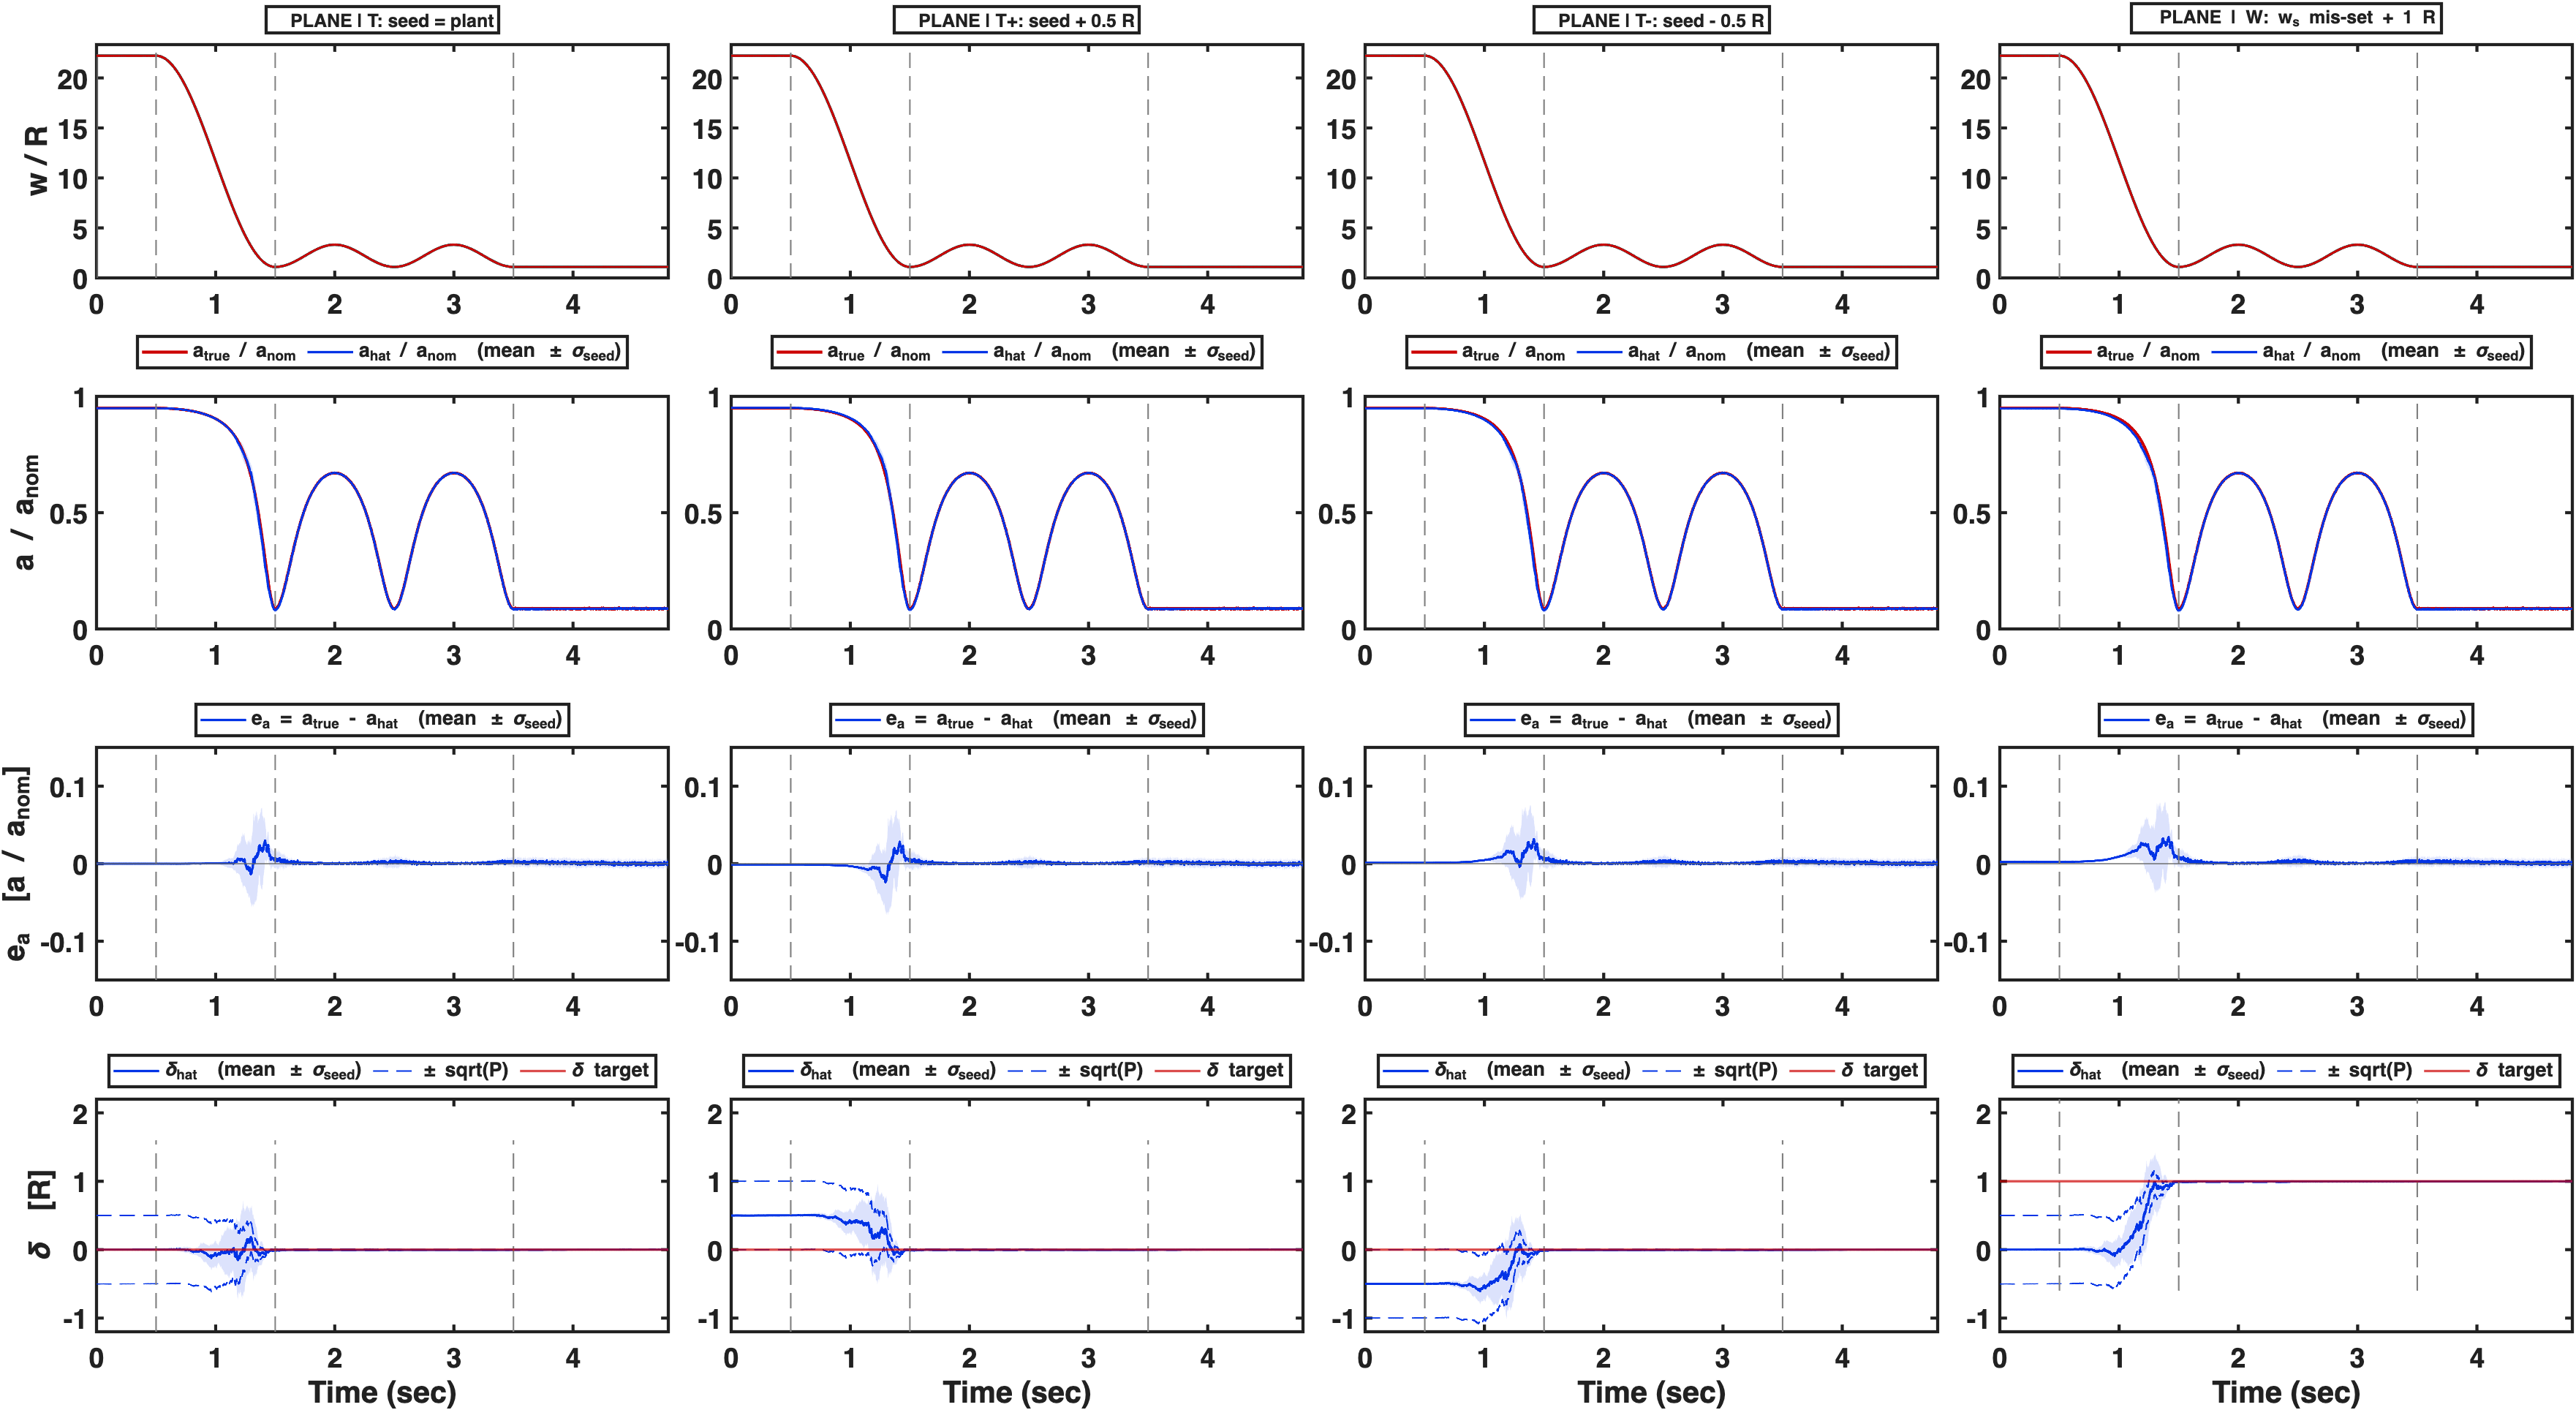
\includegraphics[width=0.93\linewidth]{figures/ladder_delta_plane.png}
\vspace*{\fill}
\end{landscape}

\begin{landscape}
\vspace*{\fill}
\noindent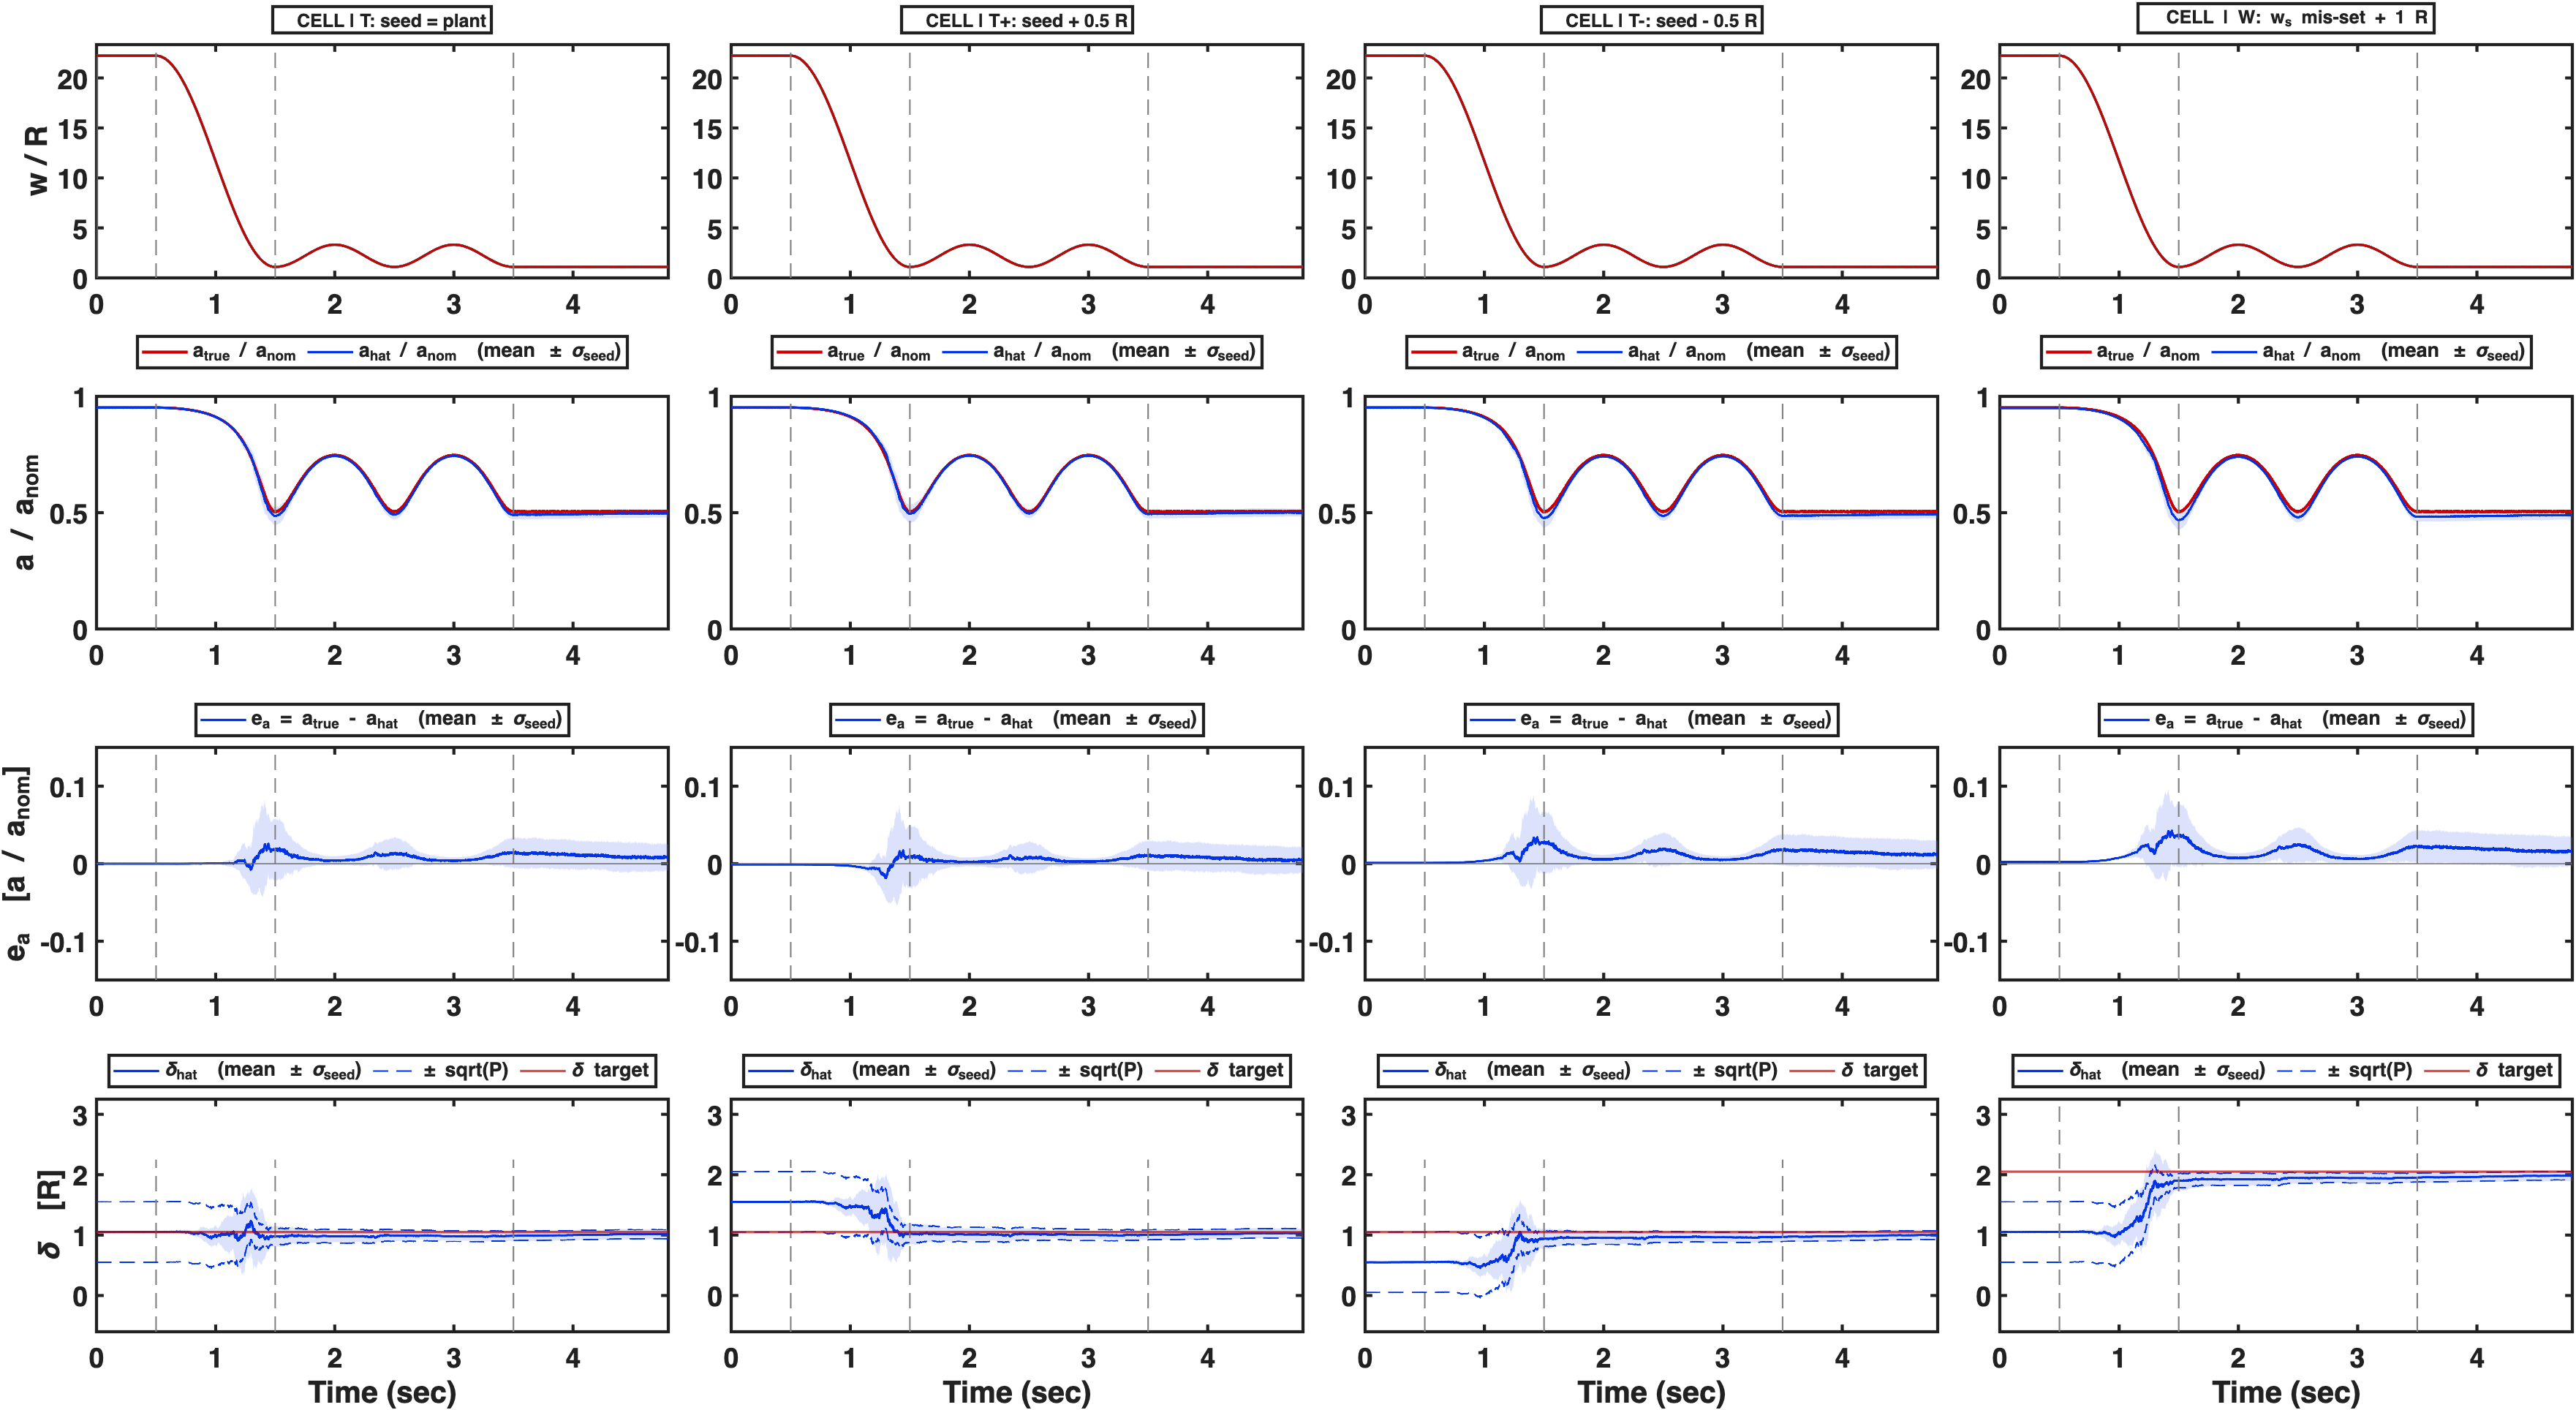
\includegraphics[width=0.93\linewidth]{figures/ladder_delta_cell.png}
\vspace*{\fill}
\end{landscape}

\clearpage
\noindent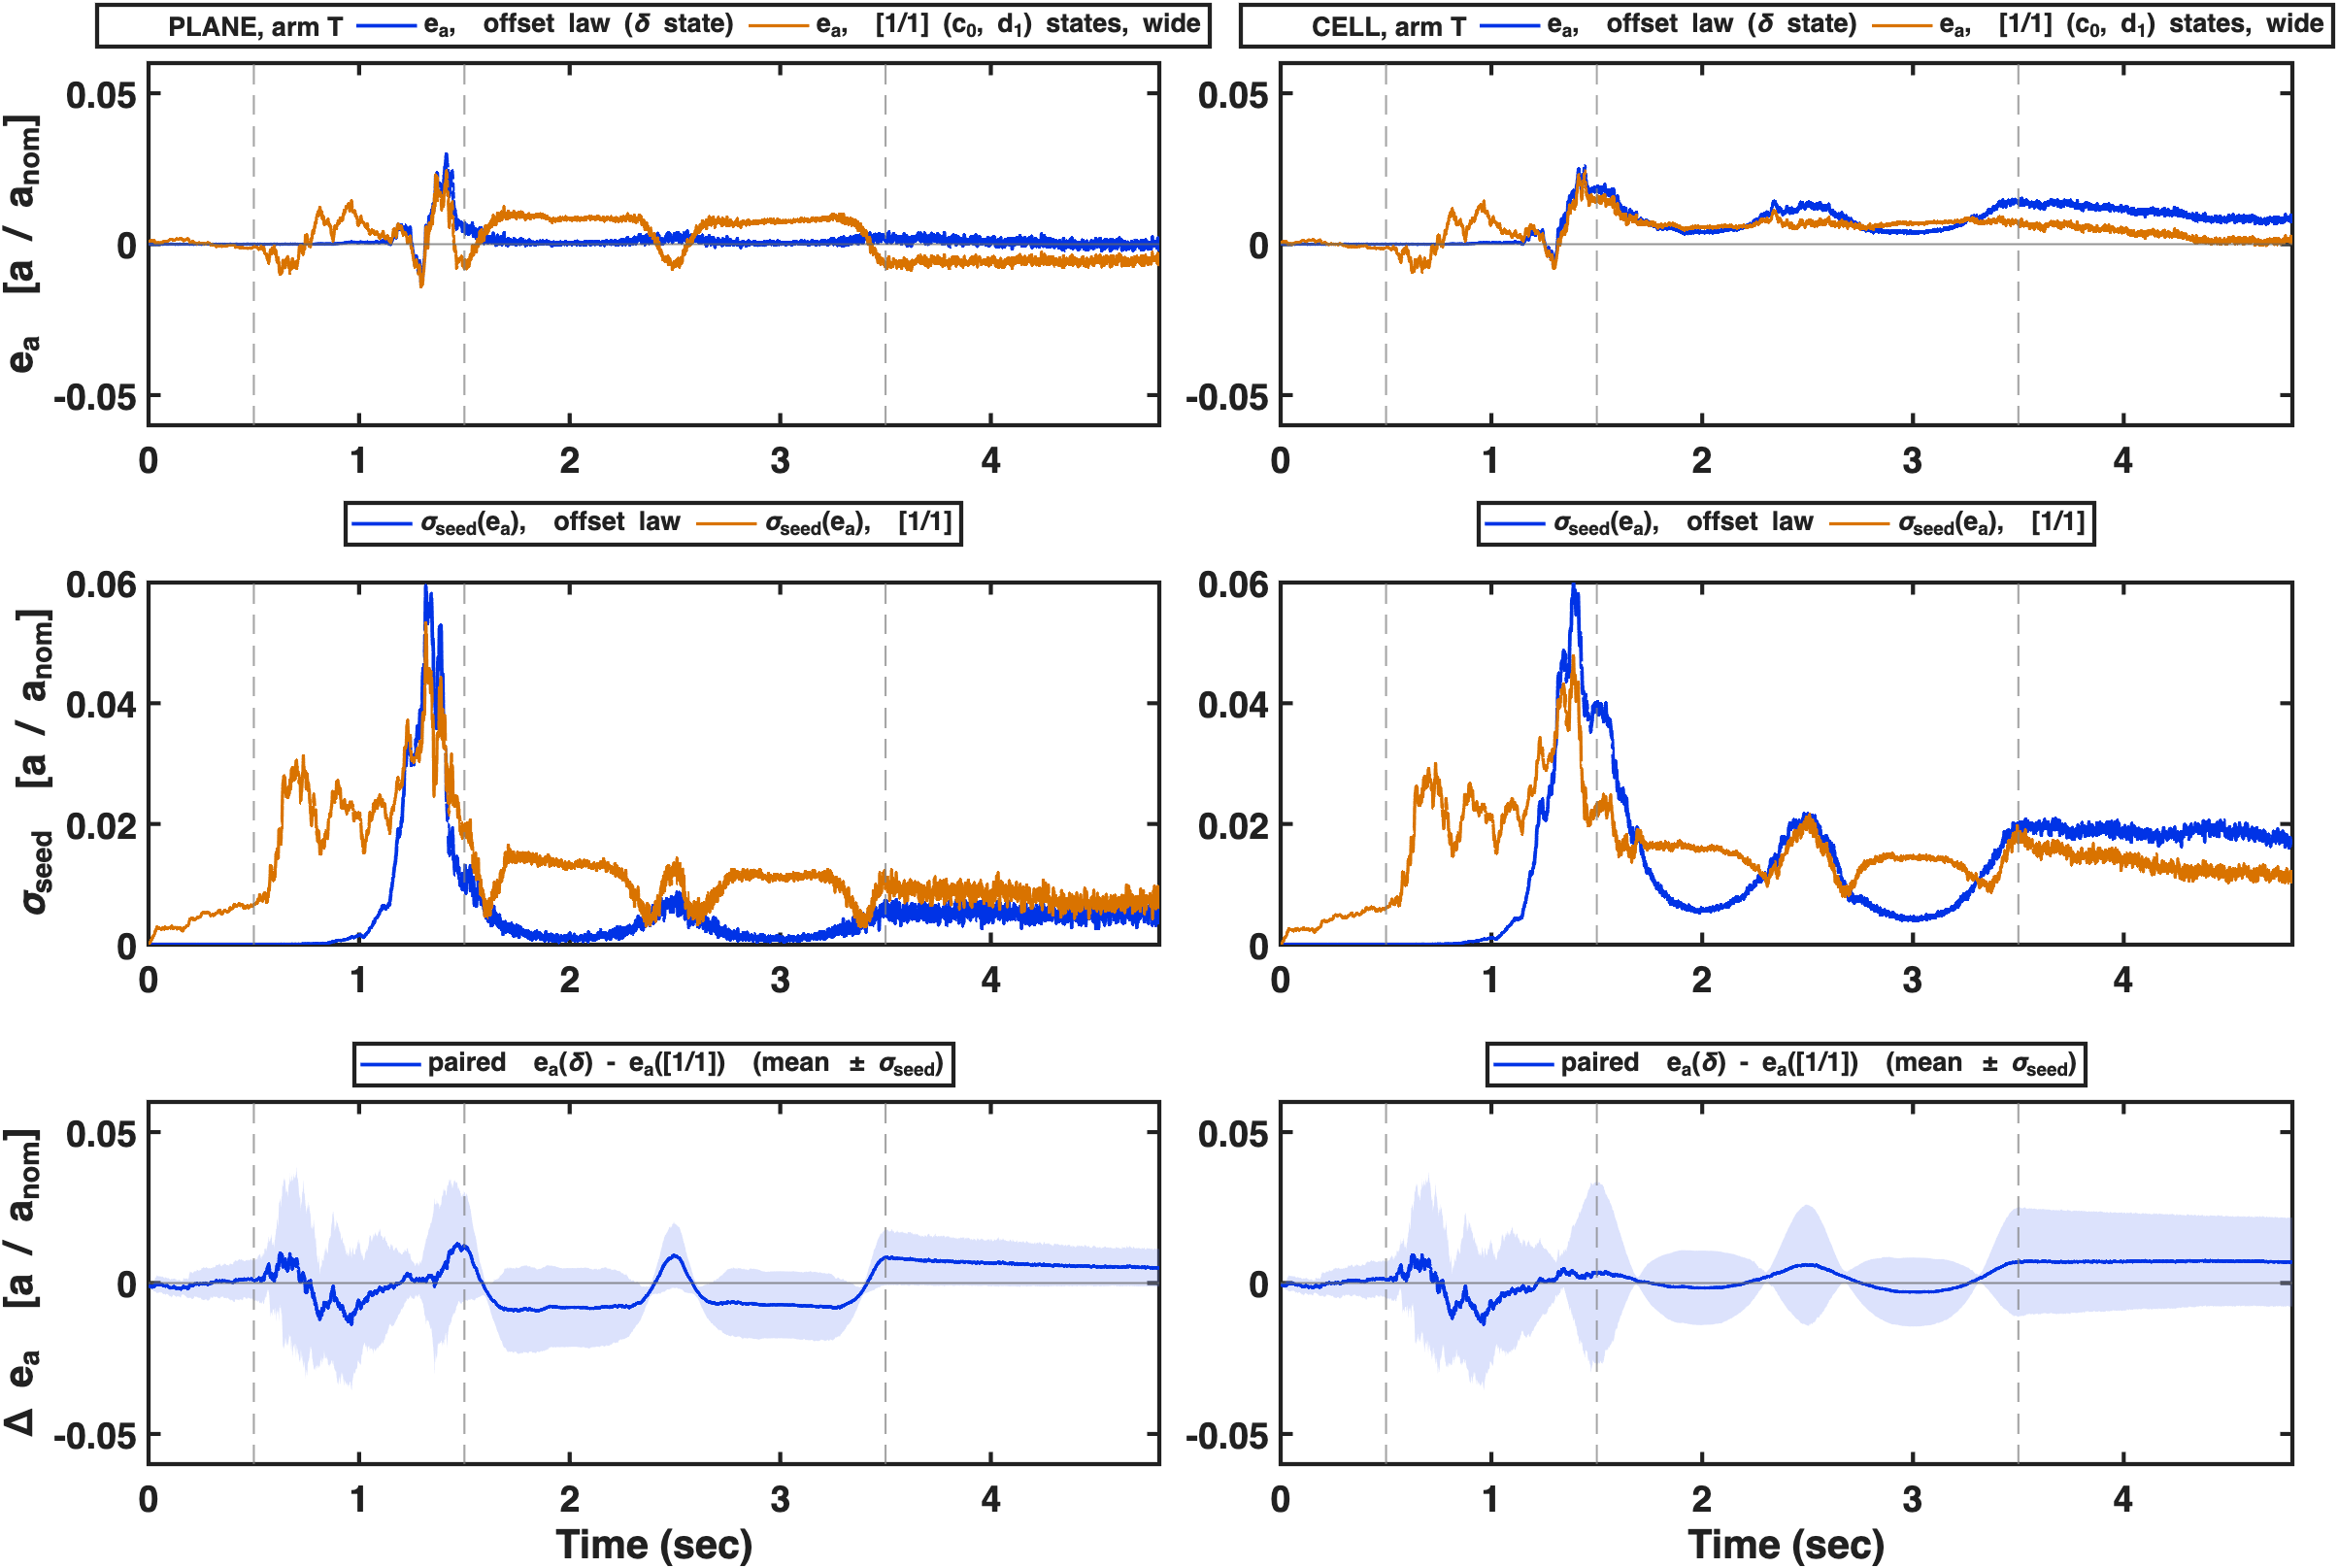
\includegraphics[width=\textwidth]{figures/delta_vs_11_T_wide.png}

\clearpage
\noindent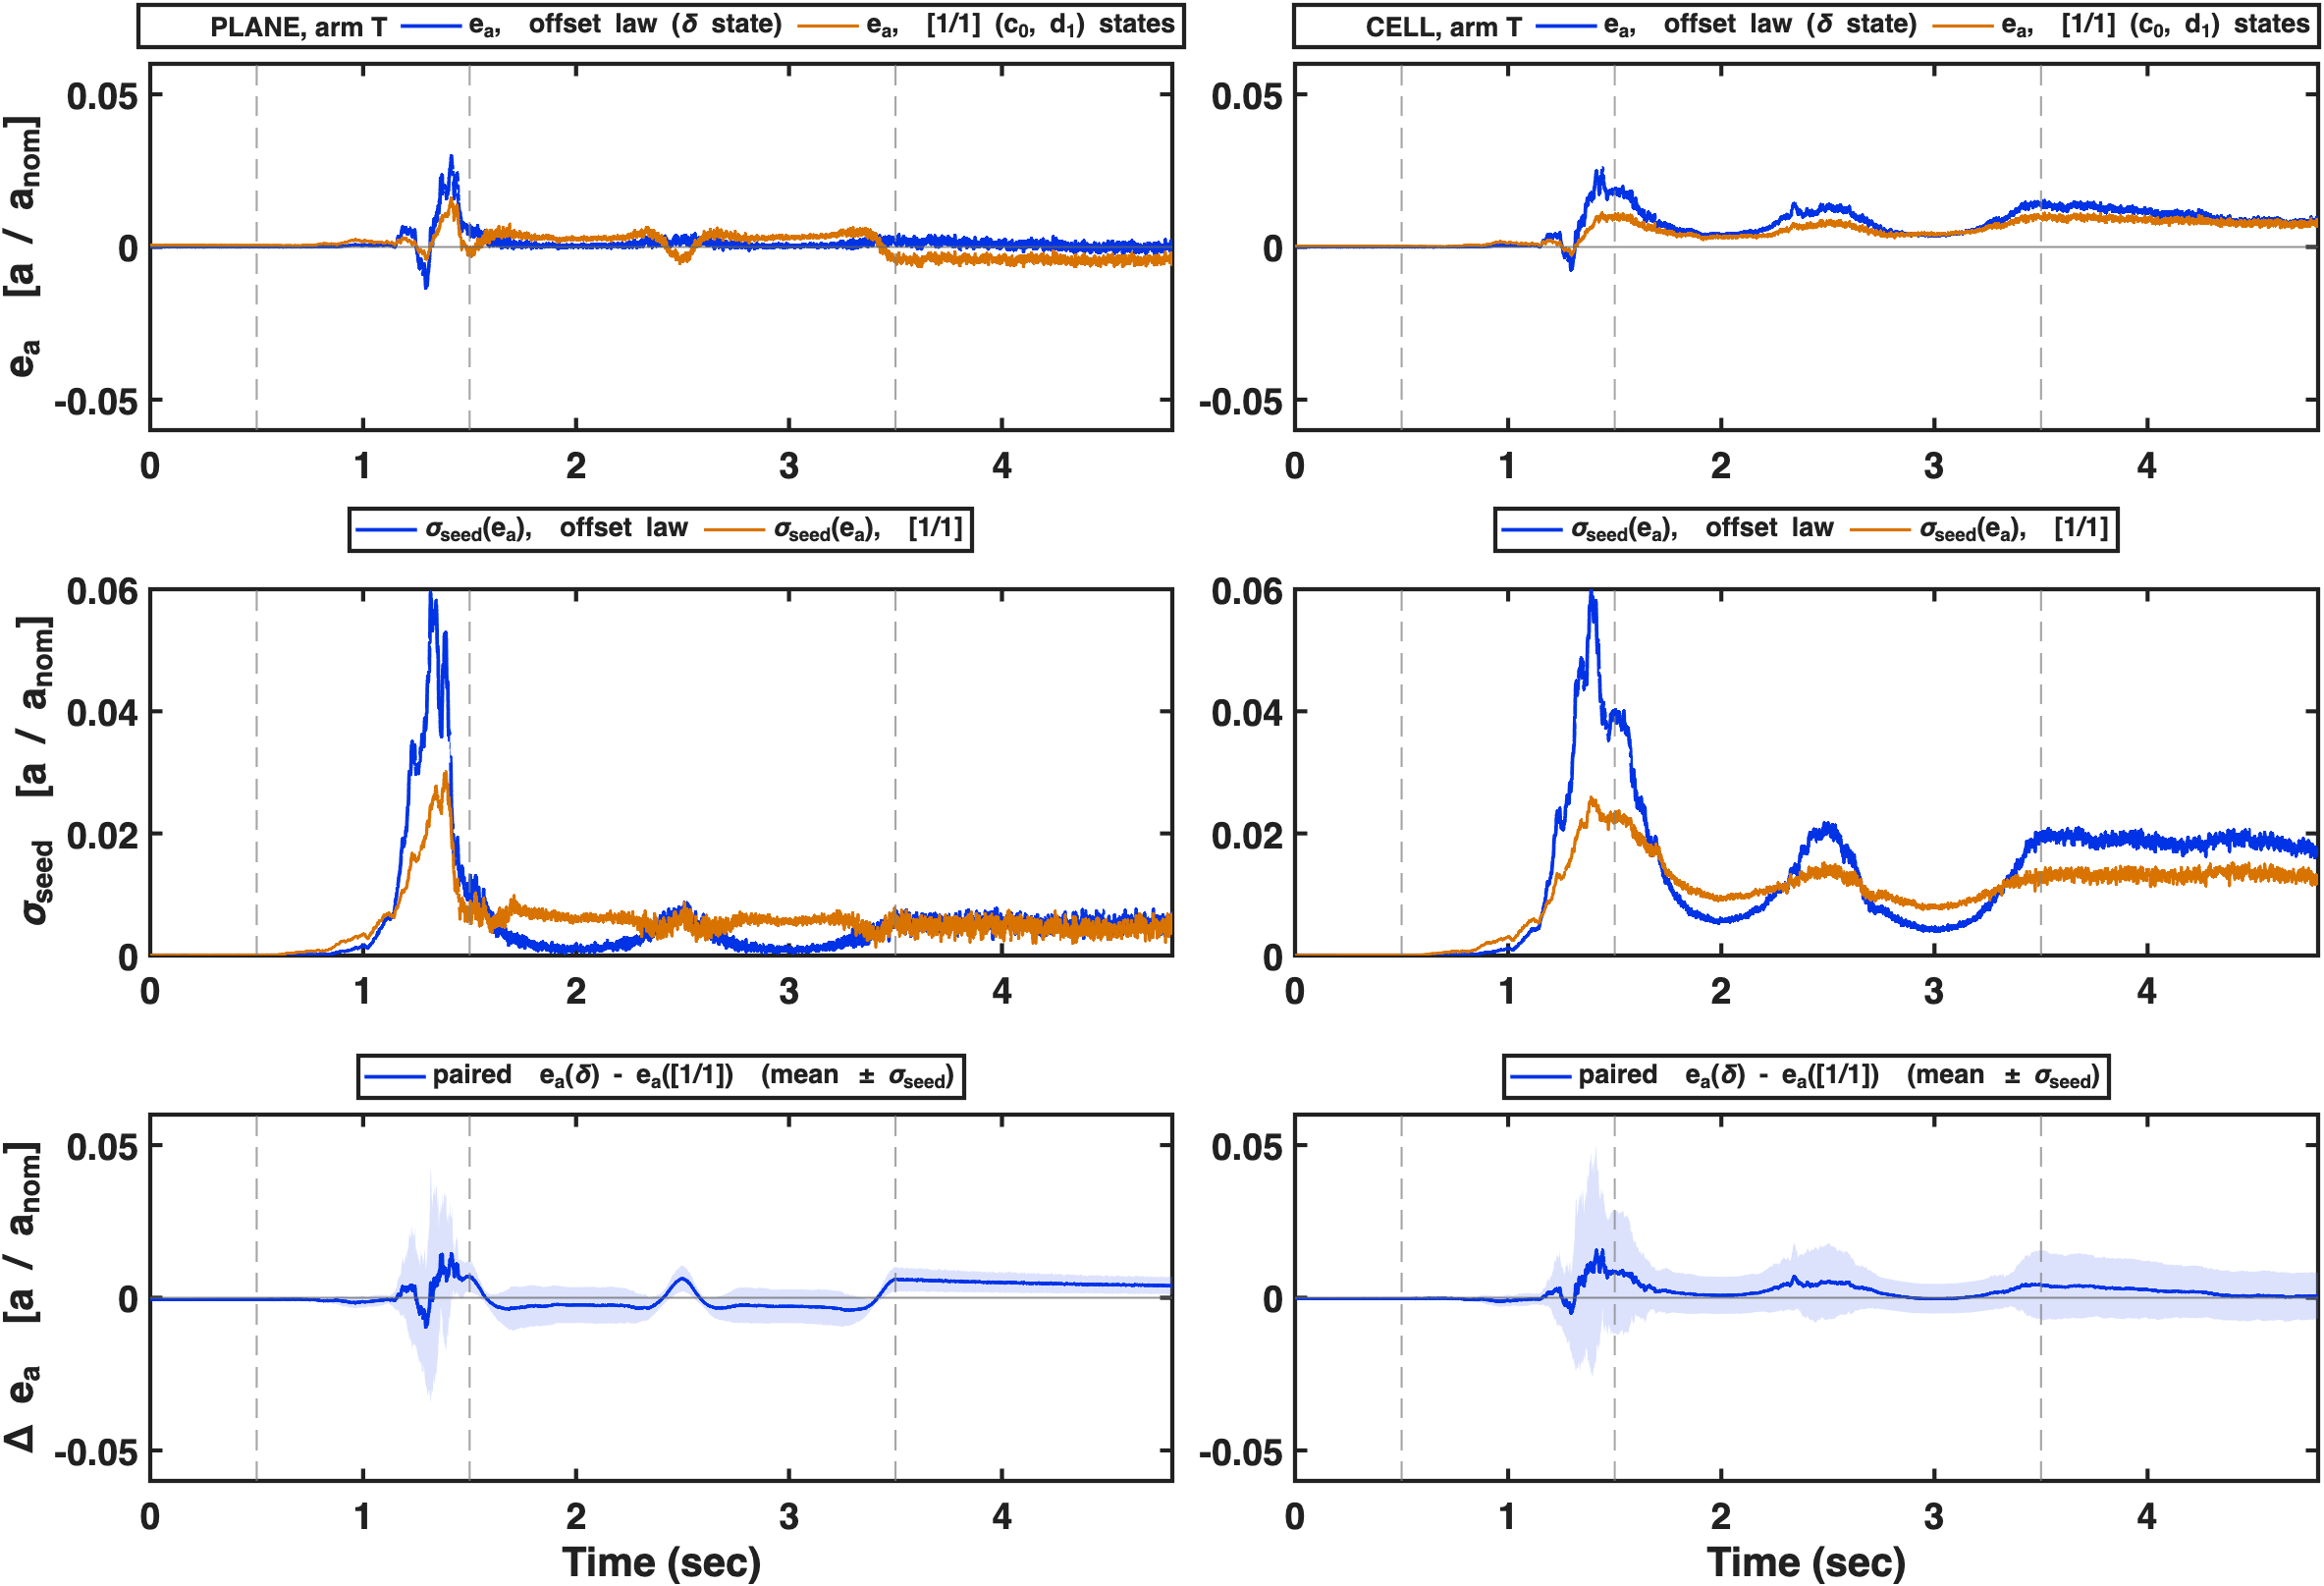
\includegraphics[width=\textwidth]{figures/delta_vs_11_T.png}

\clearpage
\centerline{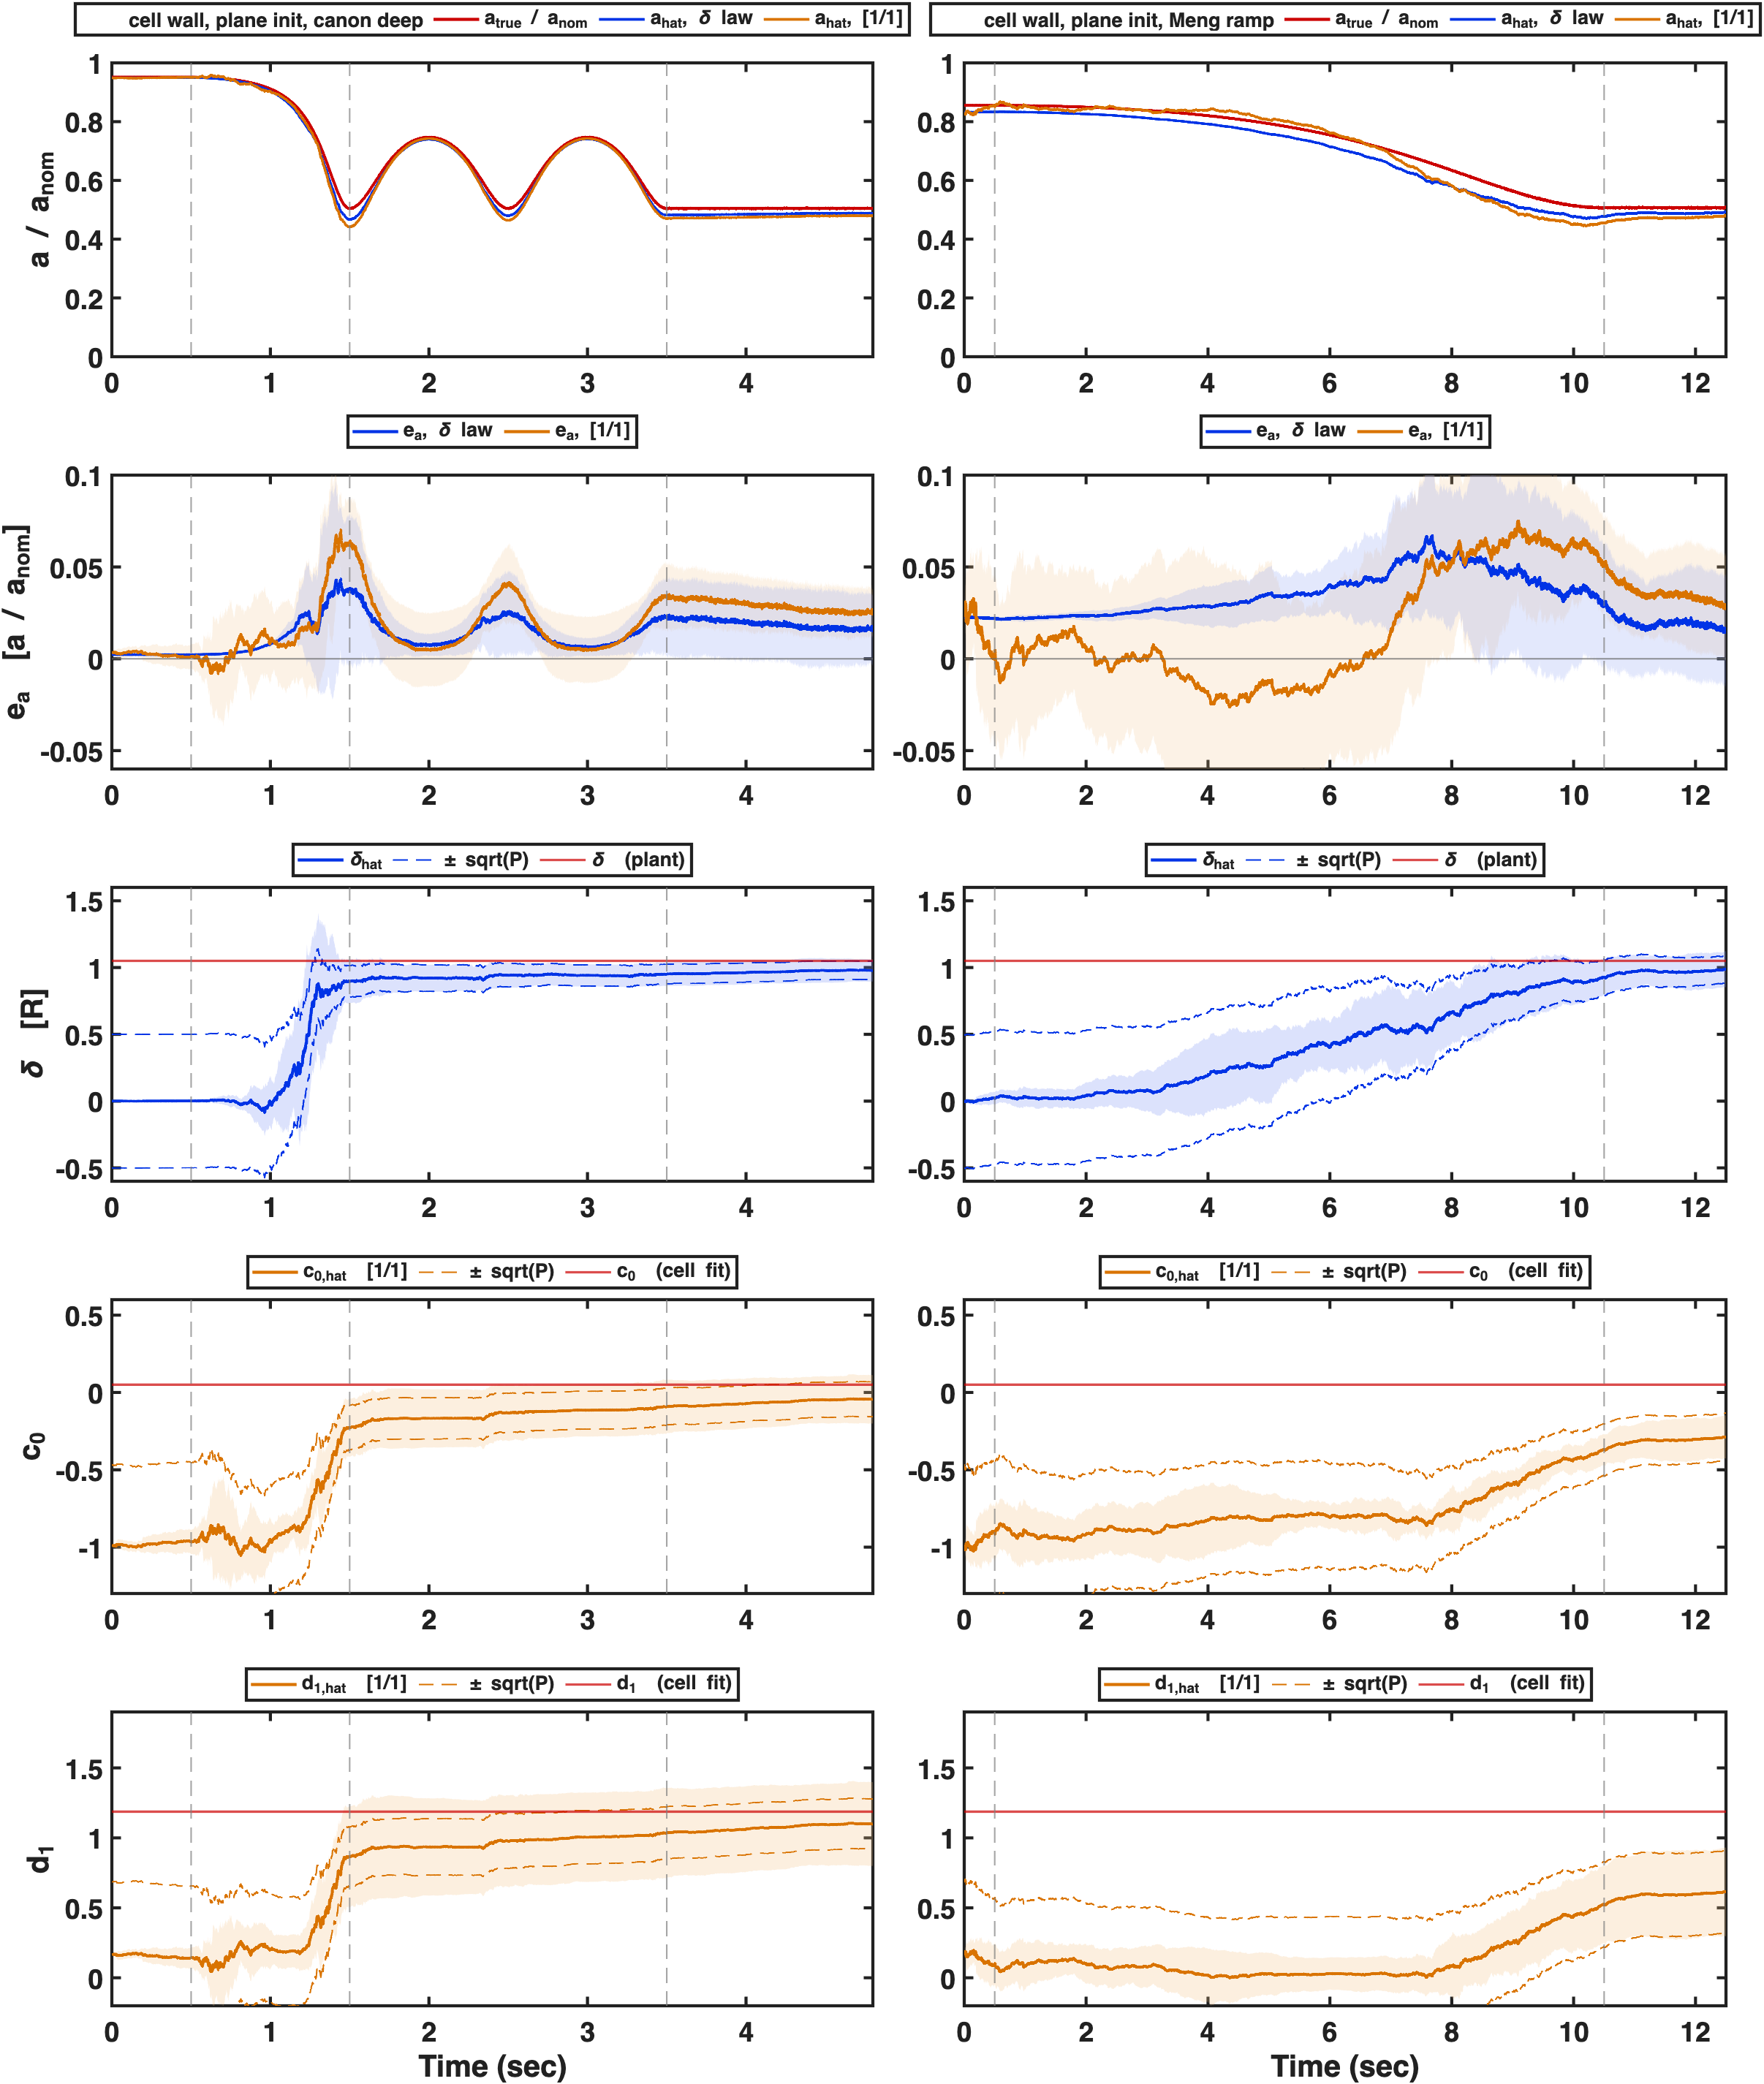
\includegraphics[width=\textwidth,height=0.93\textheight,keepaspectratio]{figures/delta_vs_11_PI.png}}

\clearpage
\centerline{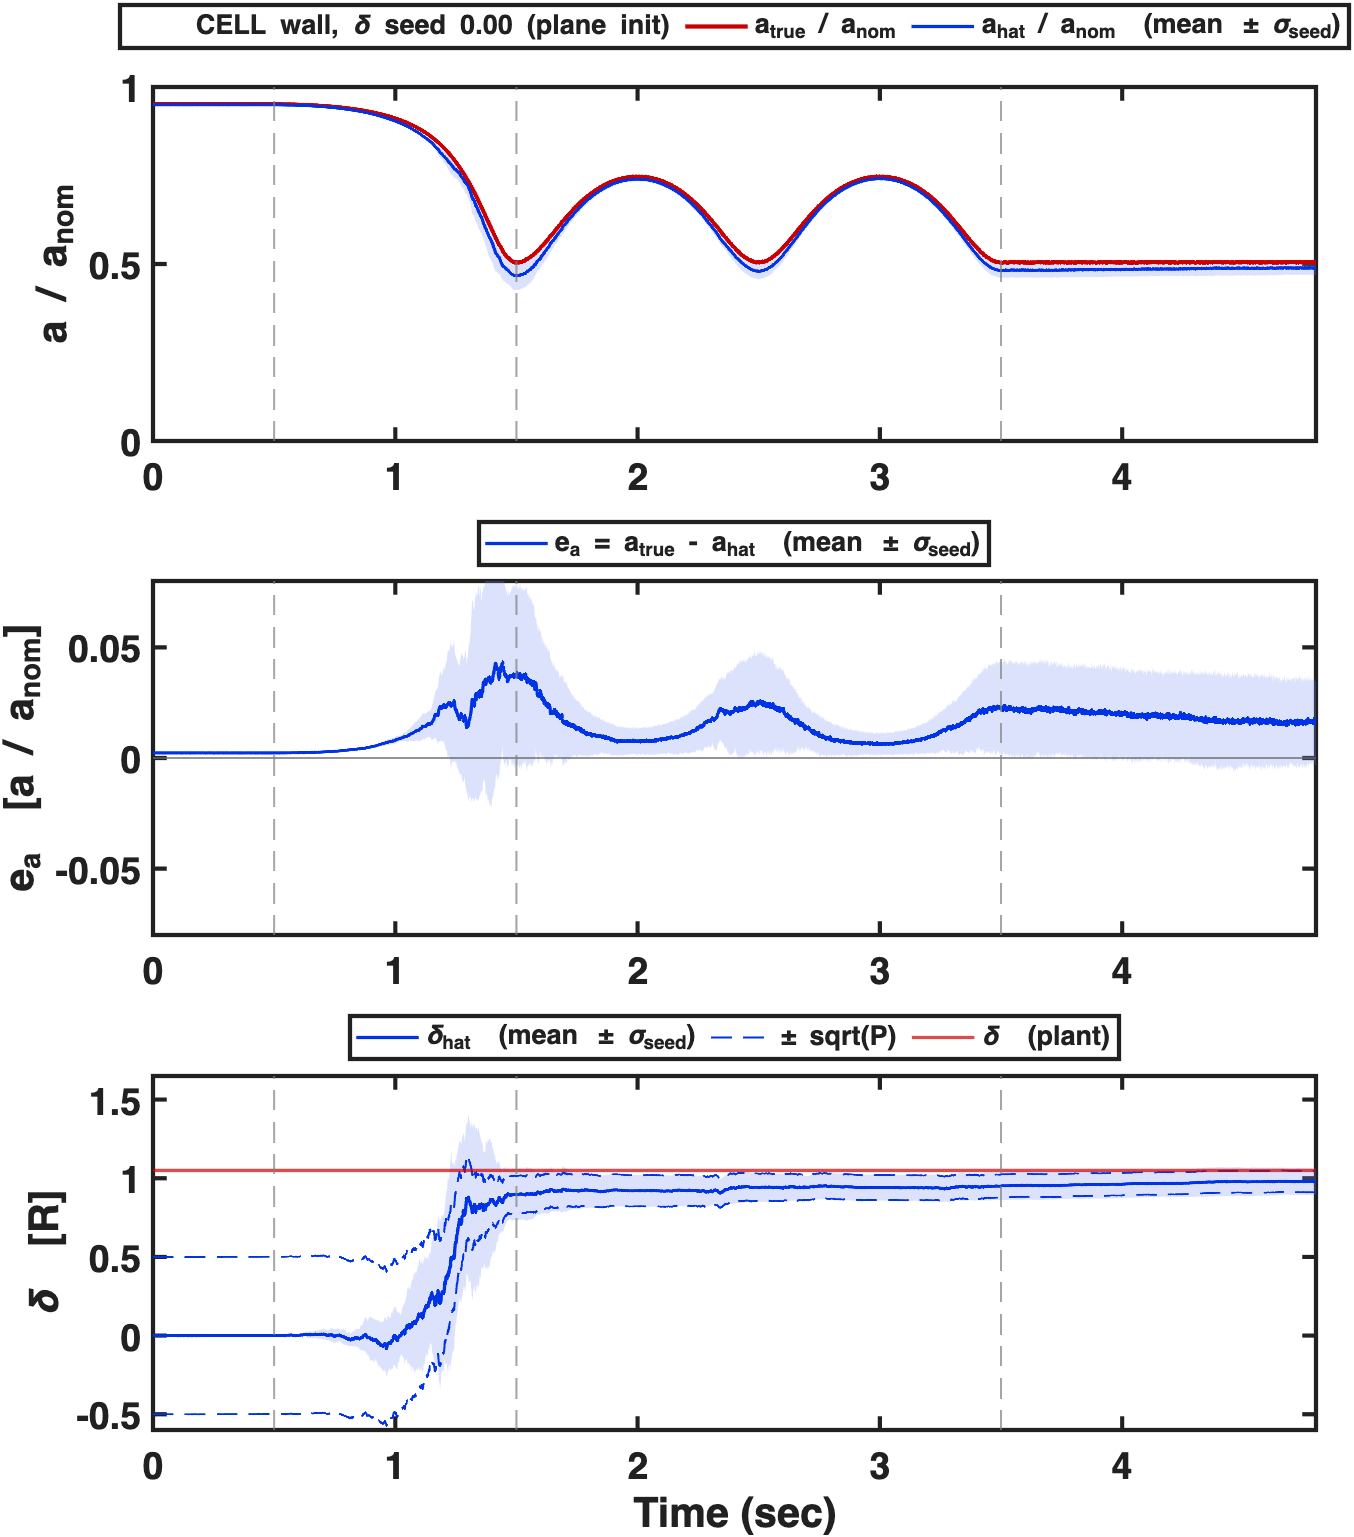
\includegraphics[width=\textwidth,height=0.93\textheight,keepaspectratio]{figures/ladder_delta_compact_PI_cell.png}}

\begin{landscape}
\vspace*{\fill}
\noindent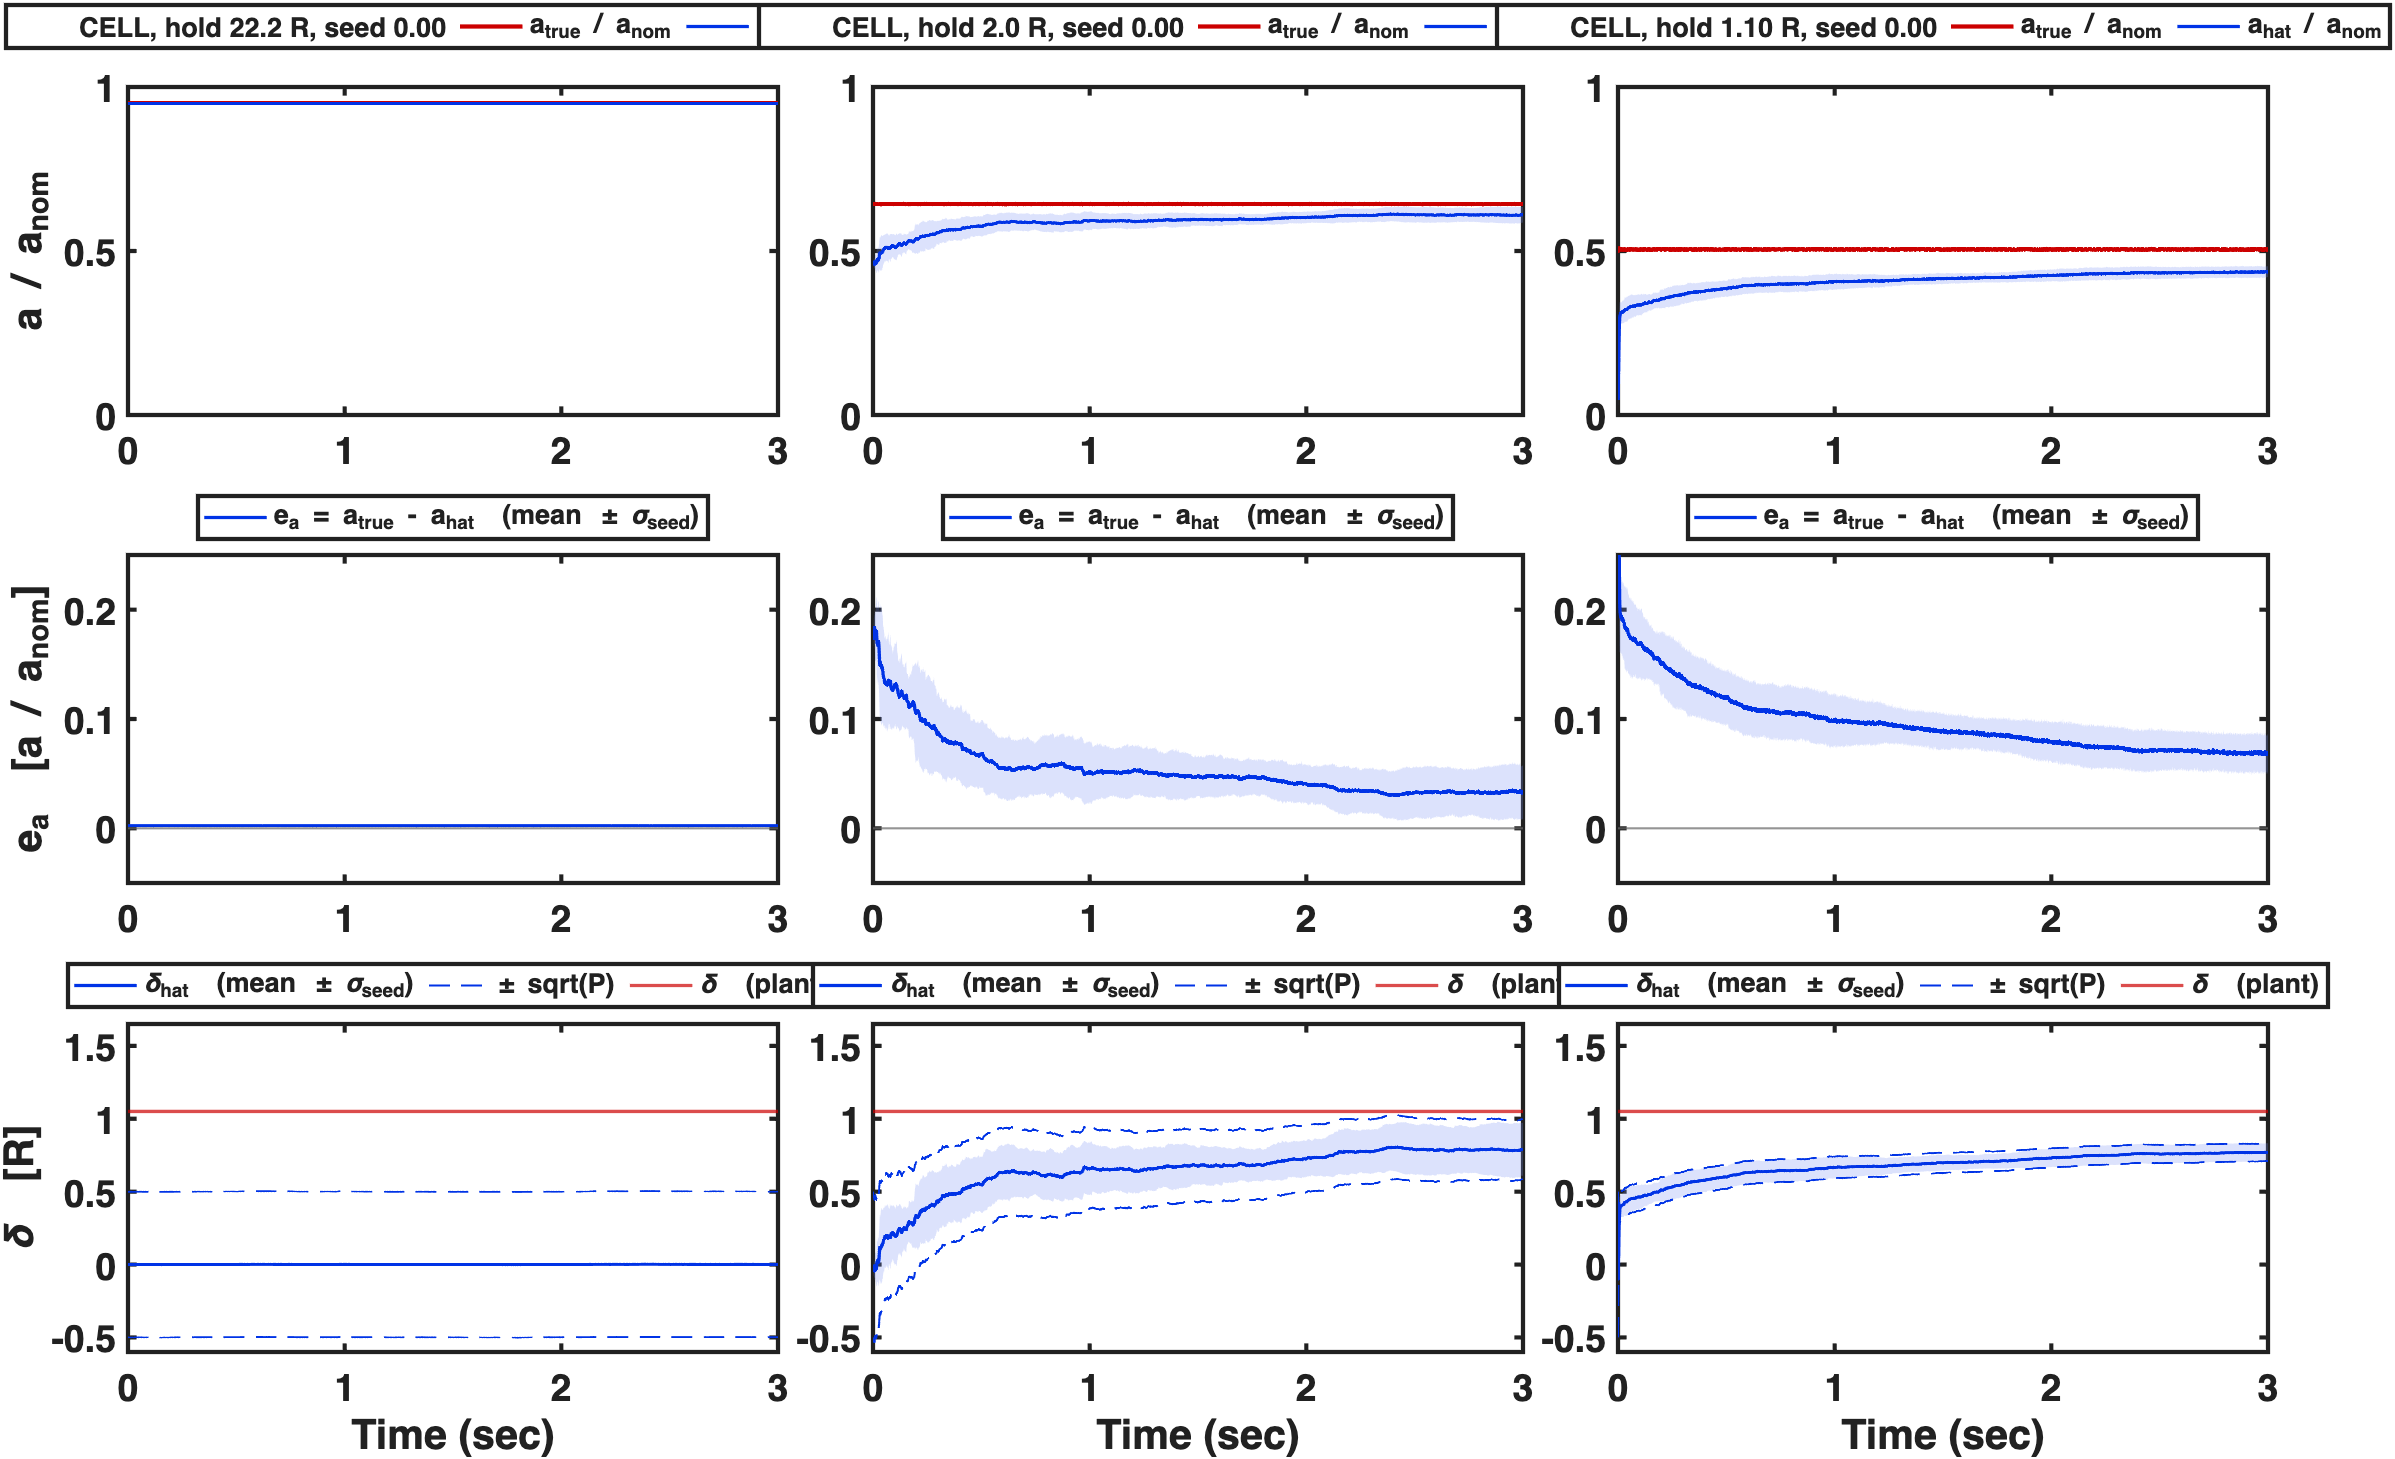
\includegraphics[width=0.93\linewidth]{figures/fixed_delta_cell_PI.png}
\vspace*{\fill}
\end{landscape}

\clearpage
\centerline{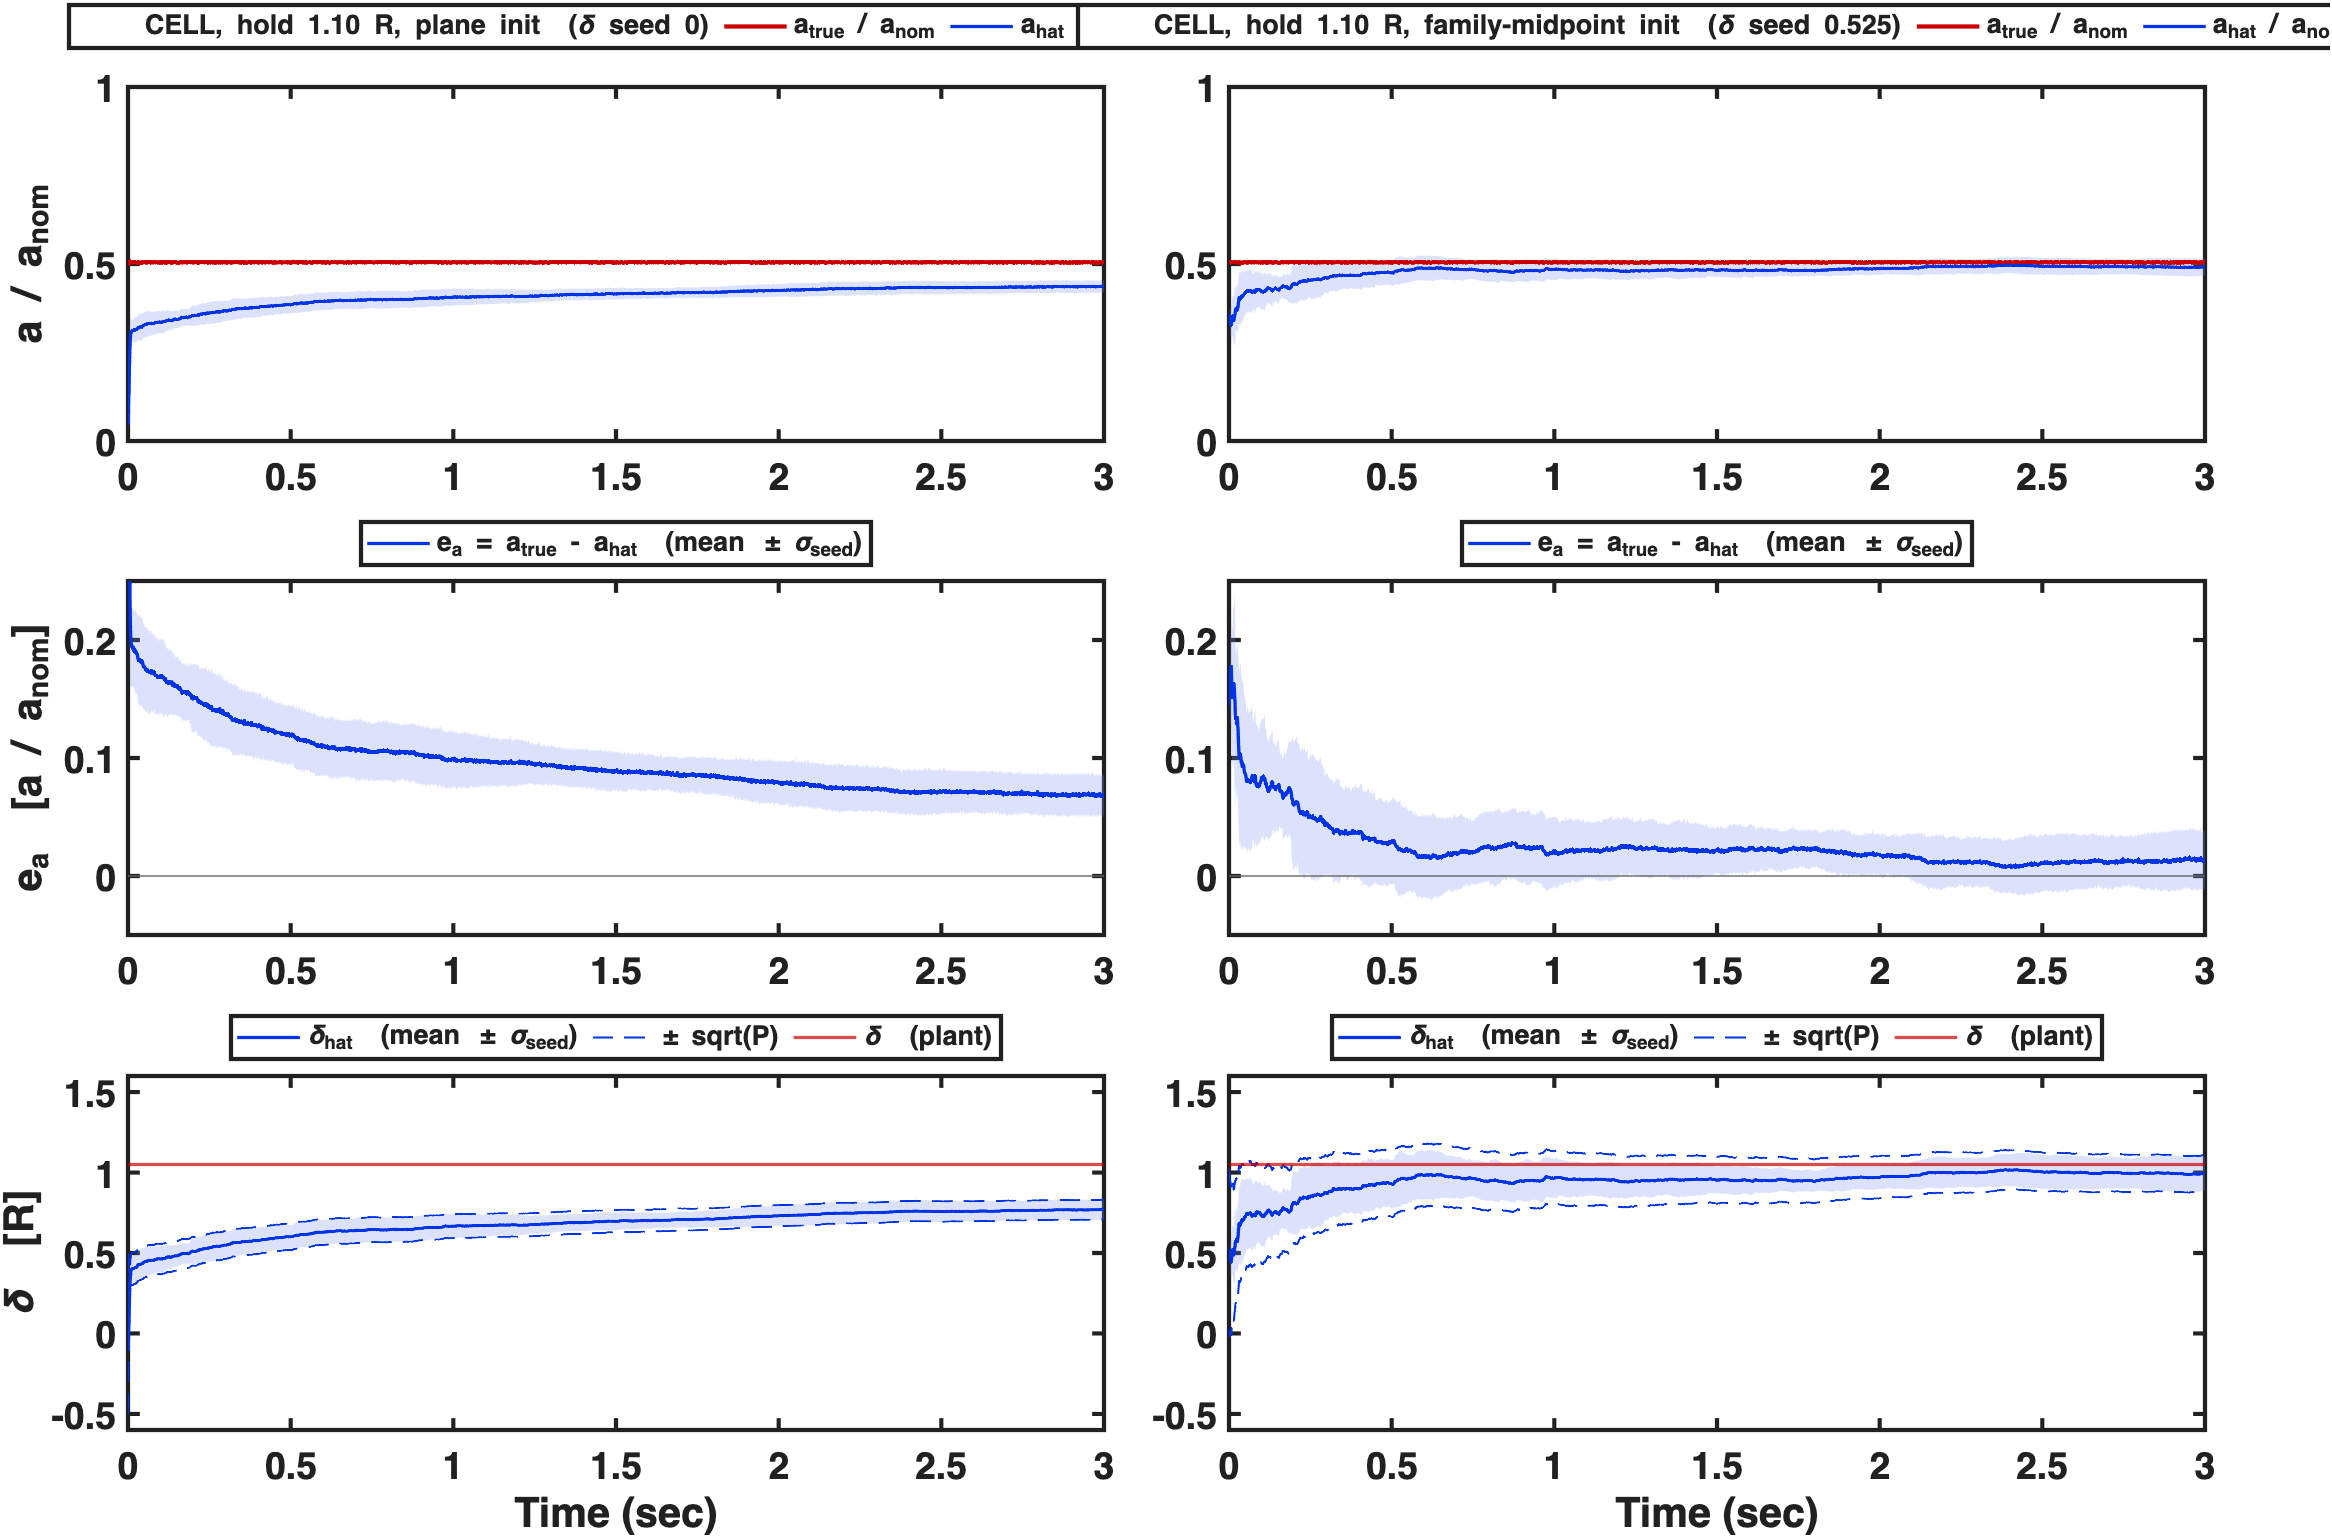
\includegraphics[width=\textwidth,height=0.93\textheight,keepaspectratio]{figures/fixed_delta_init_cell.png}}

\clearpage
\centerline{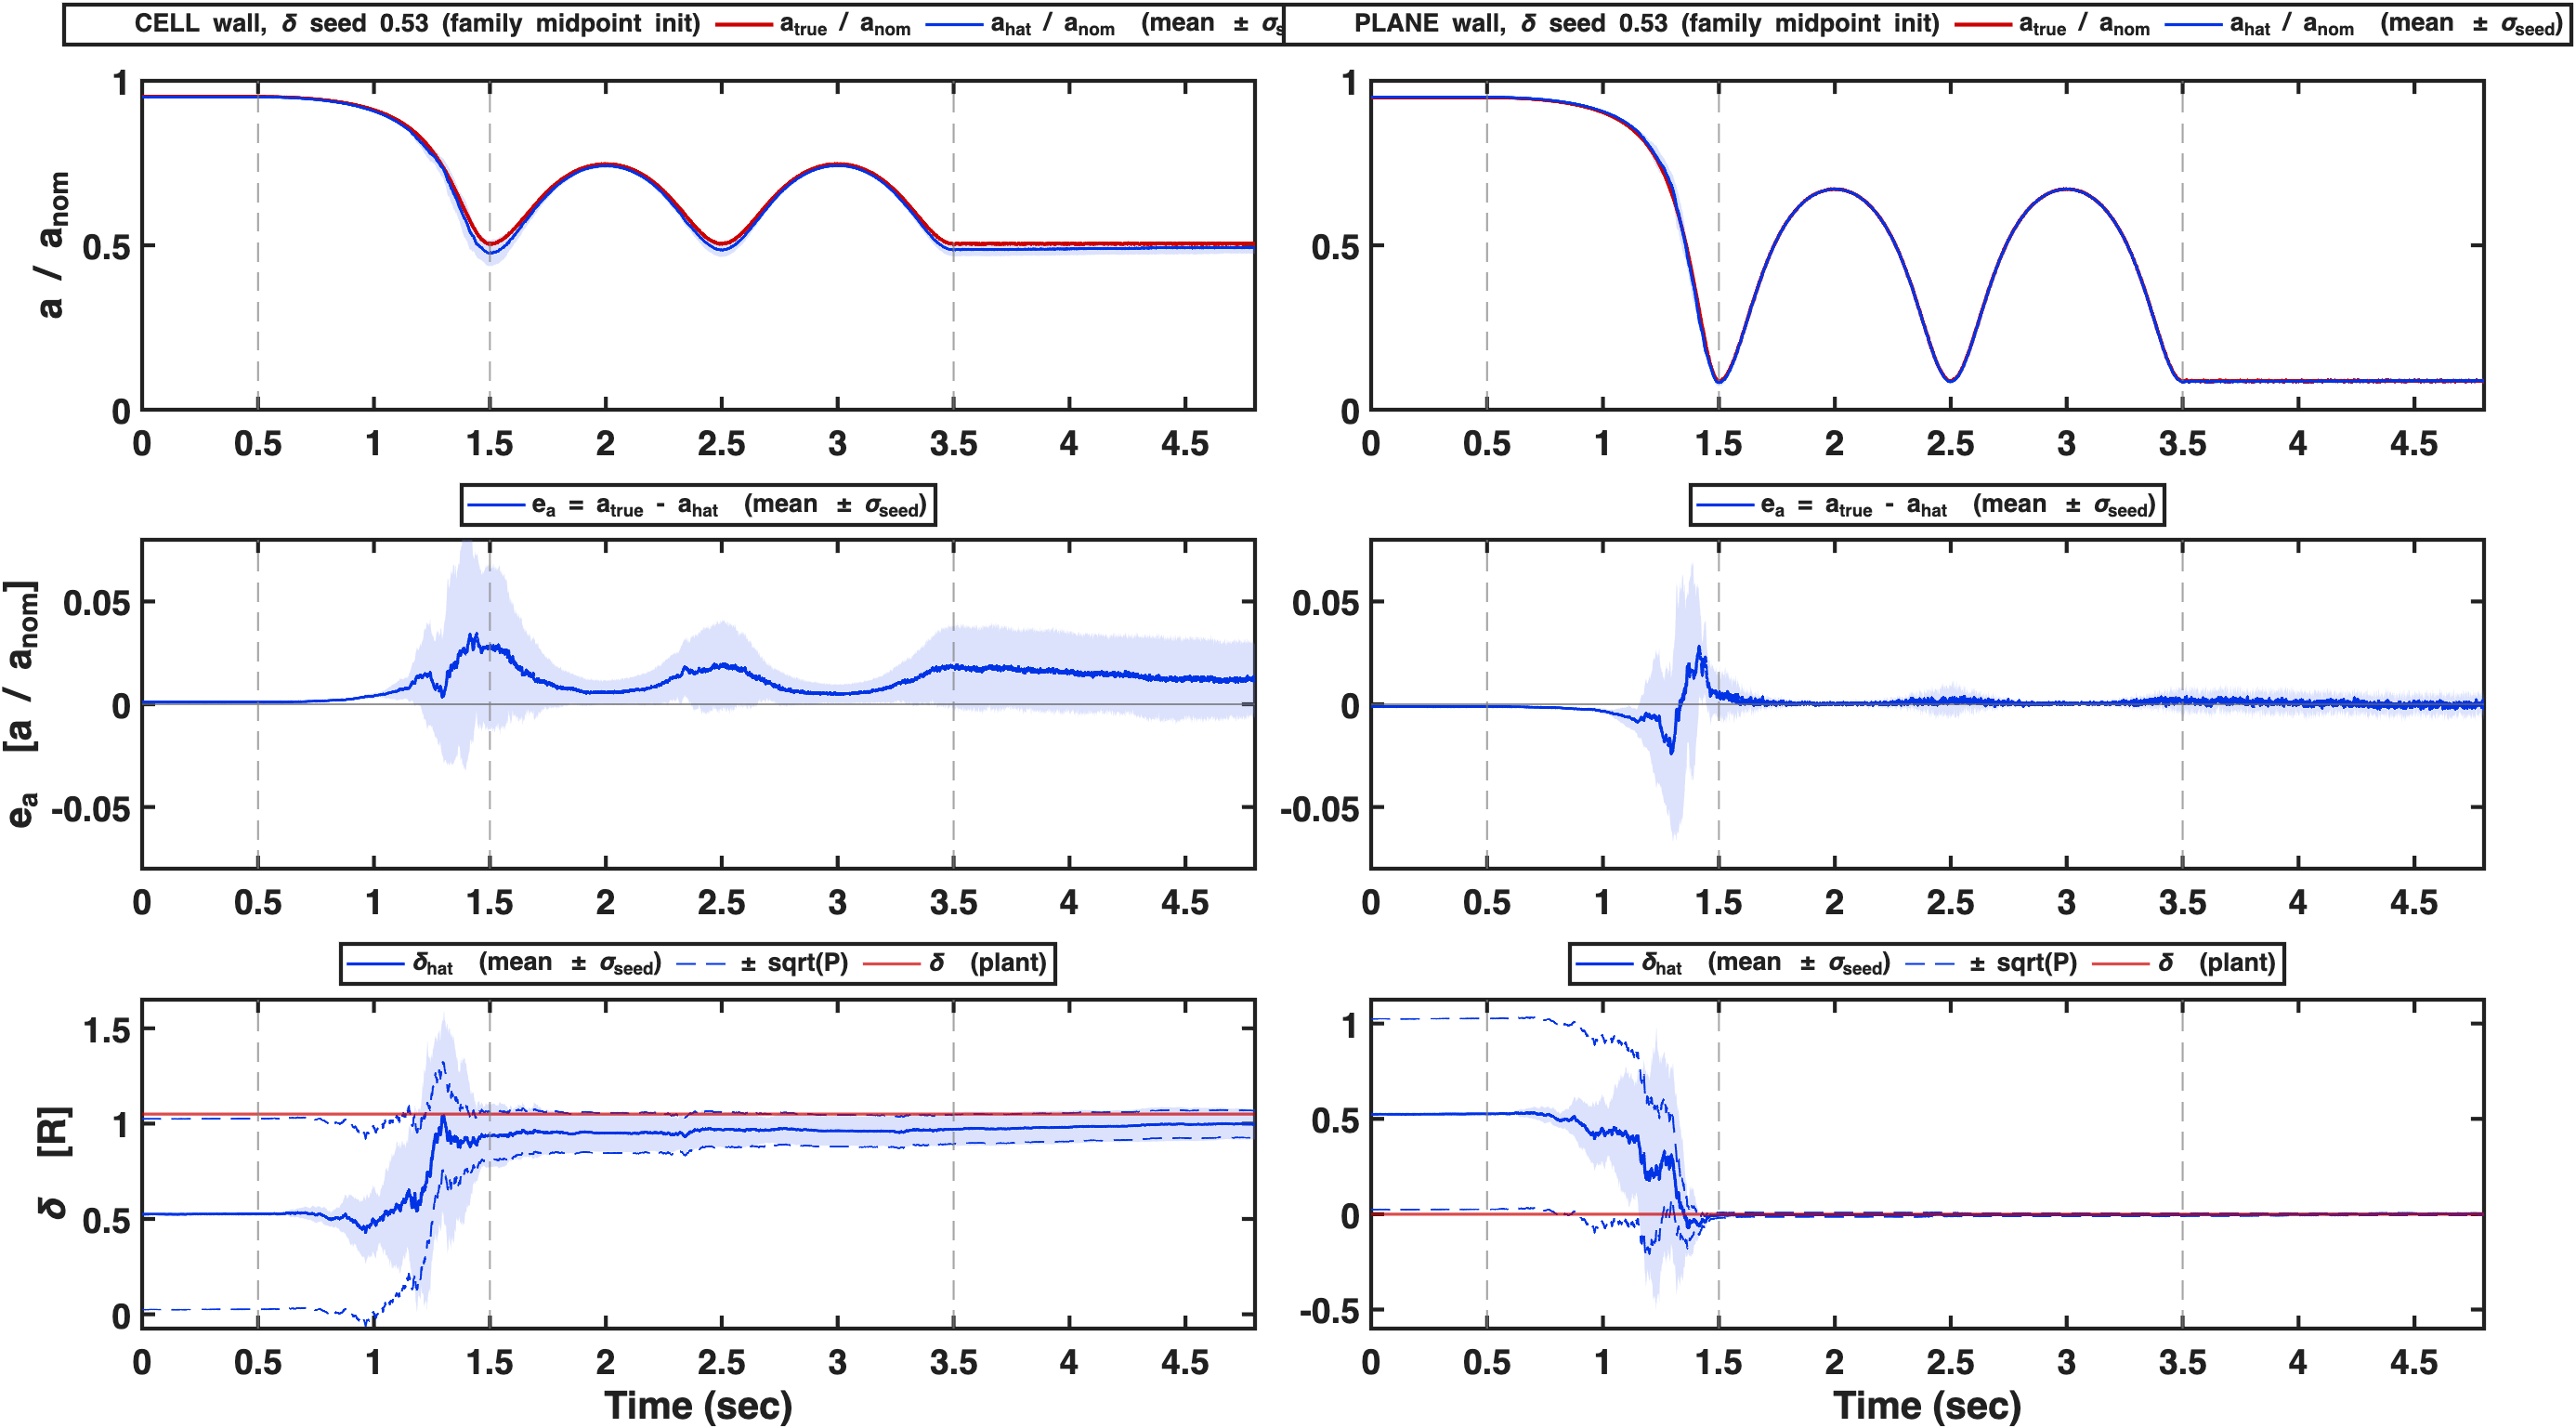
\includegraphics[width=\textwidth,height=0.93\textheight,keepaspectratio]{figures/ladder_delta_compact_MID_cell_plane.png}}

\begin{landscape}
\vspace*{\fill}
\noindent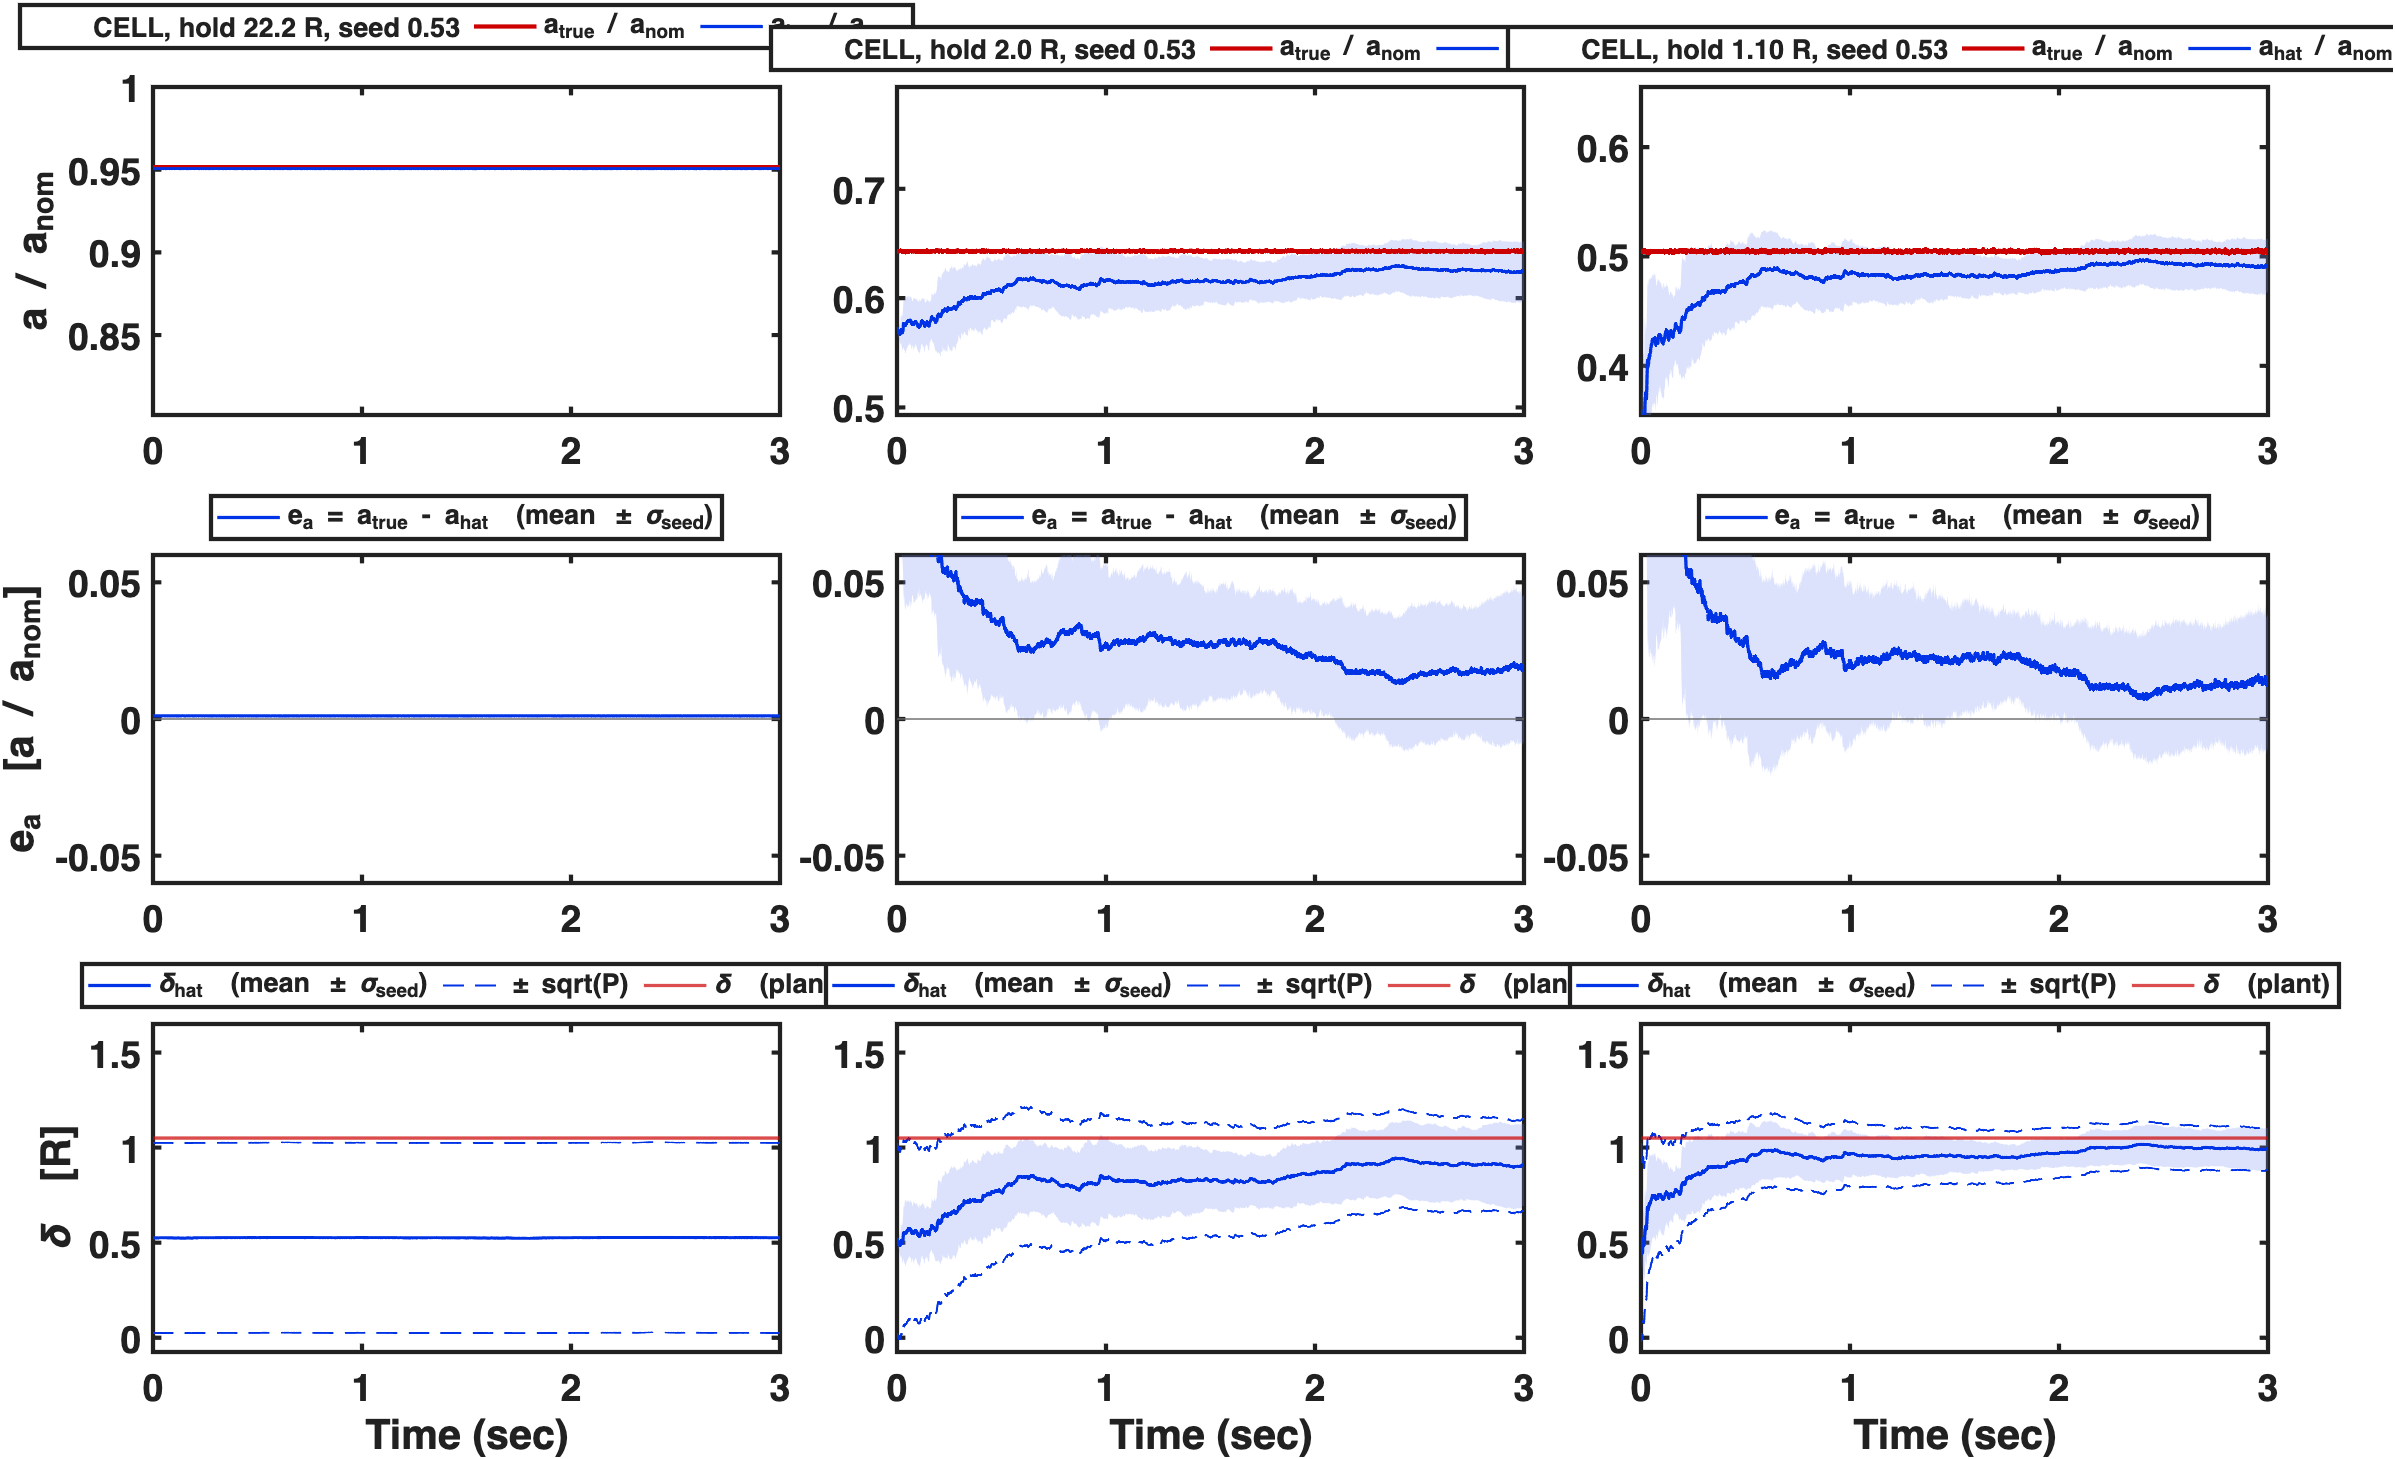
\includegraphics[width=0.93\linewidth]{figures/fixed_delta_cell_MID.png}
\vspace*{\fill}
\end{landscape}

\clearpage
\noindent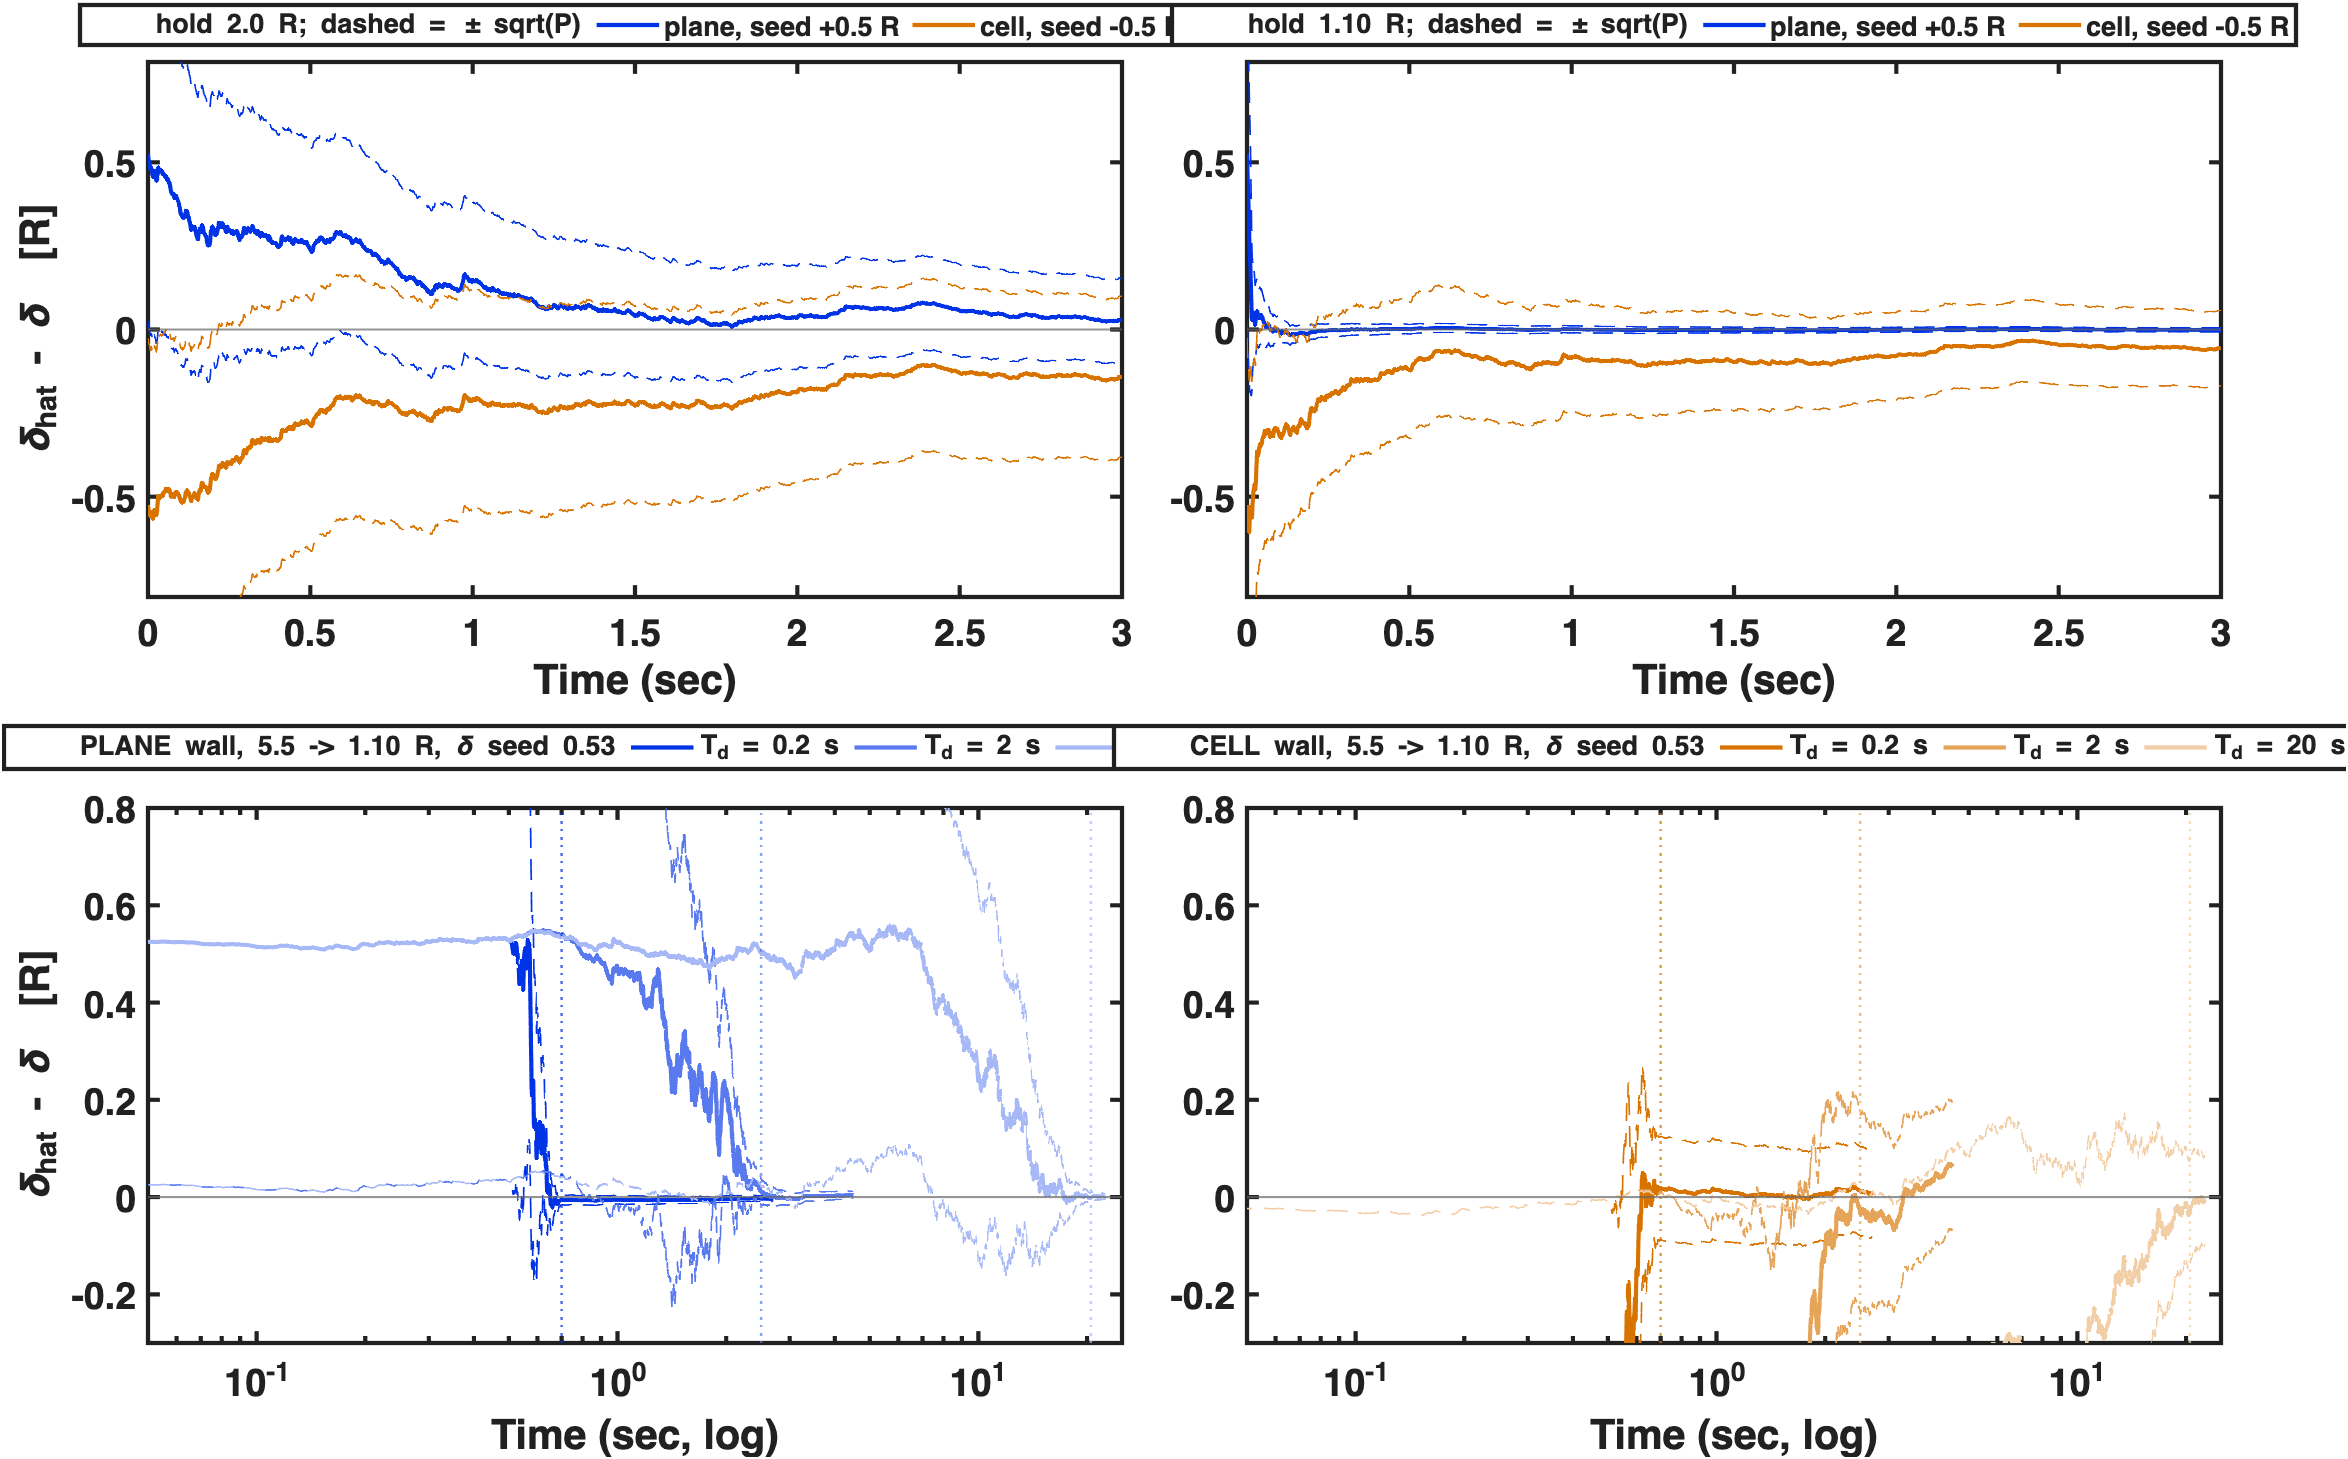
\includegraphics[width=\textwidth]{figures/delta_fixed_speed_MID.png}

\clearpage
\noindent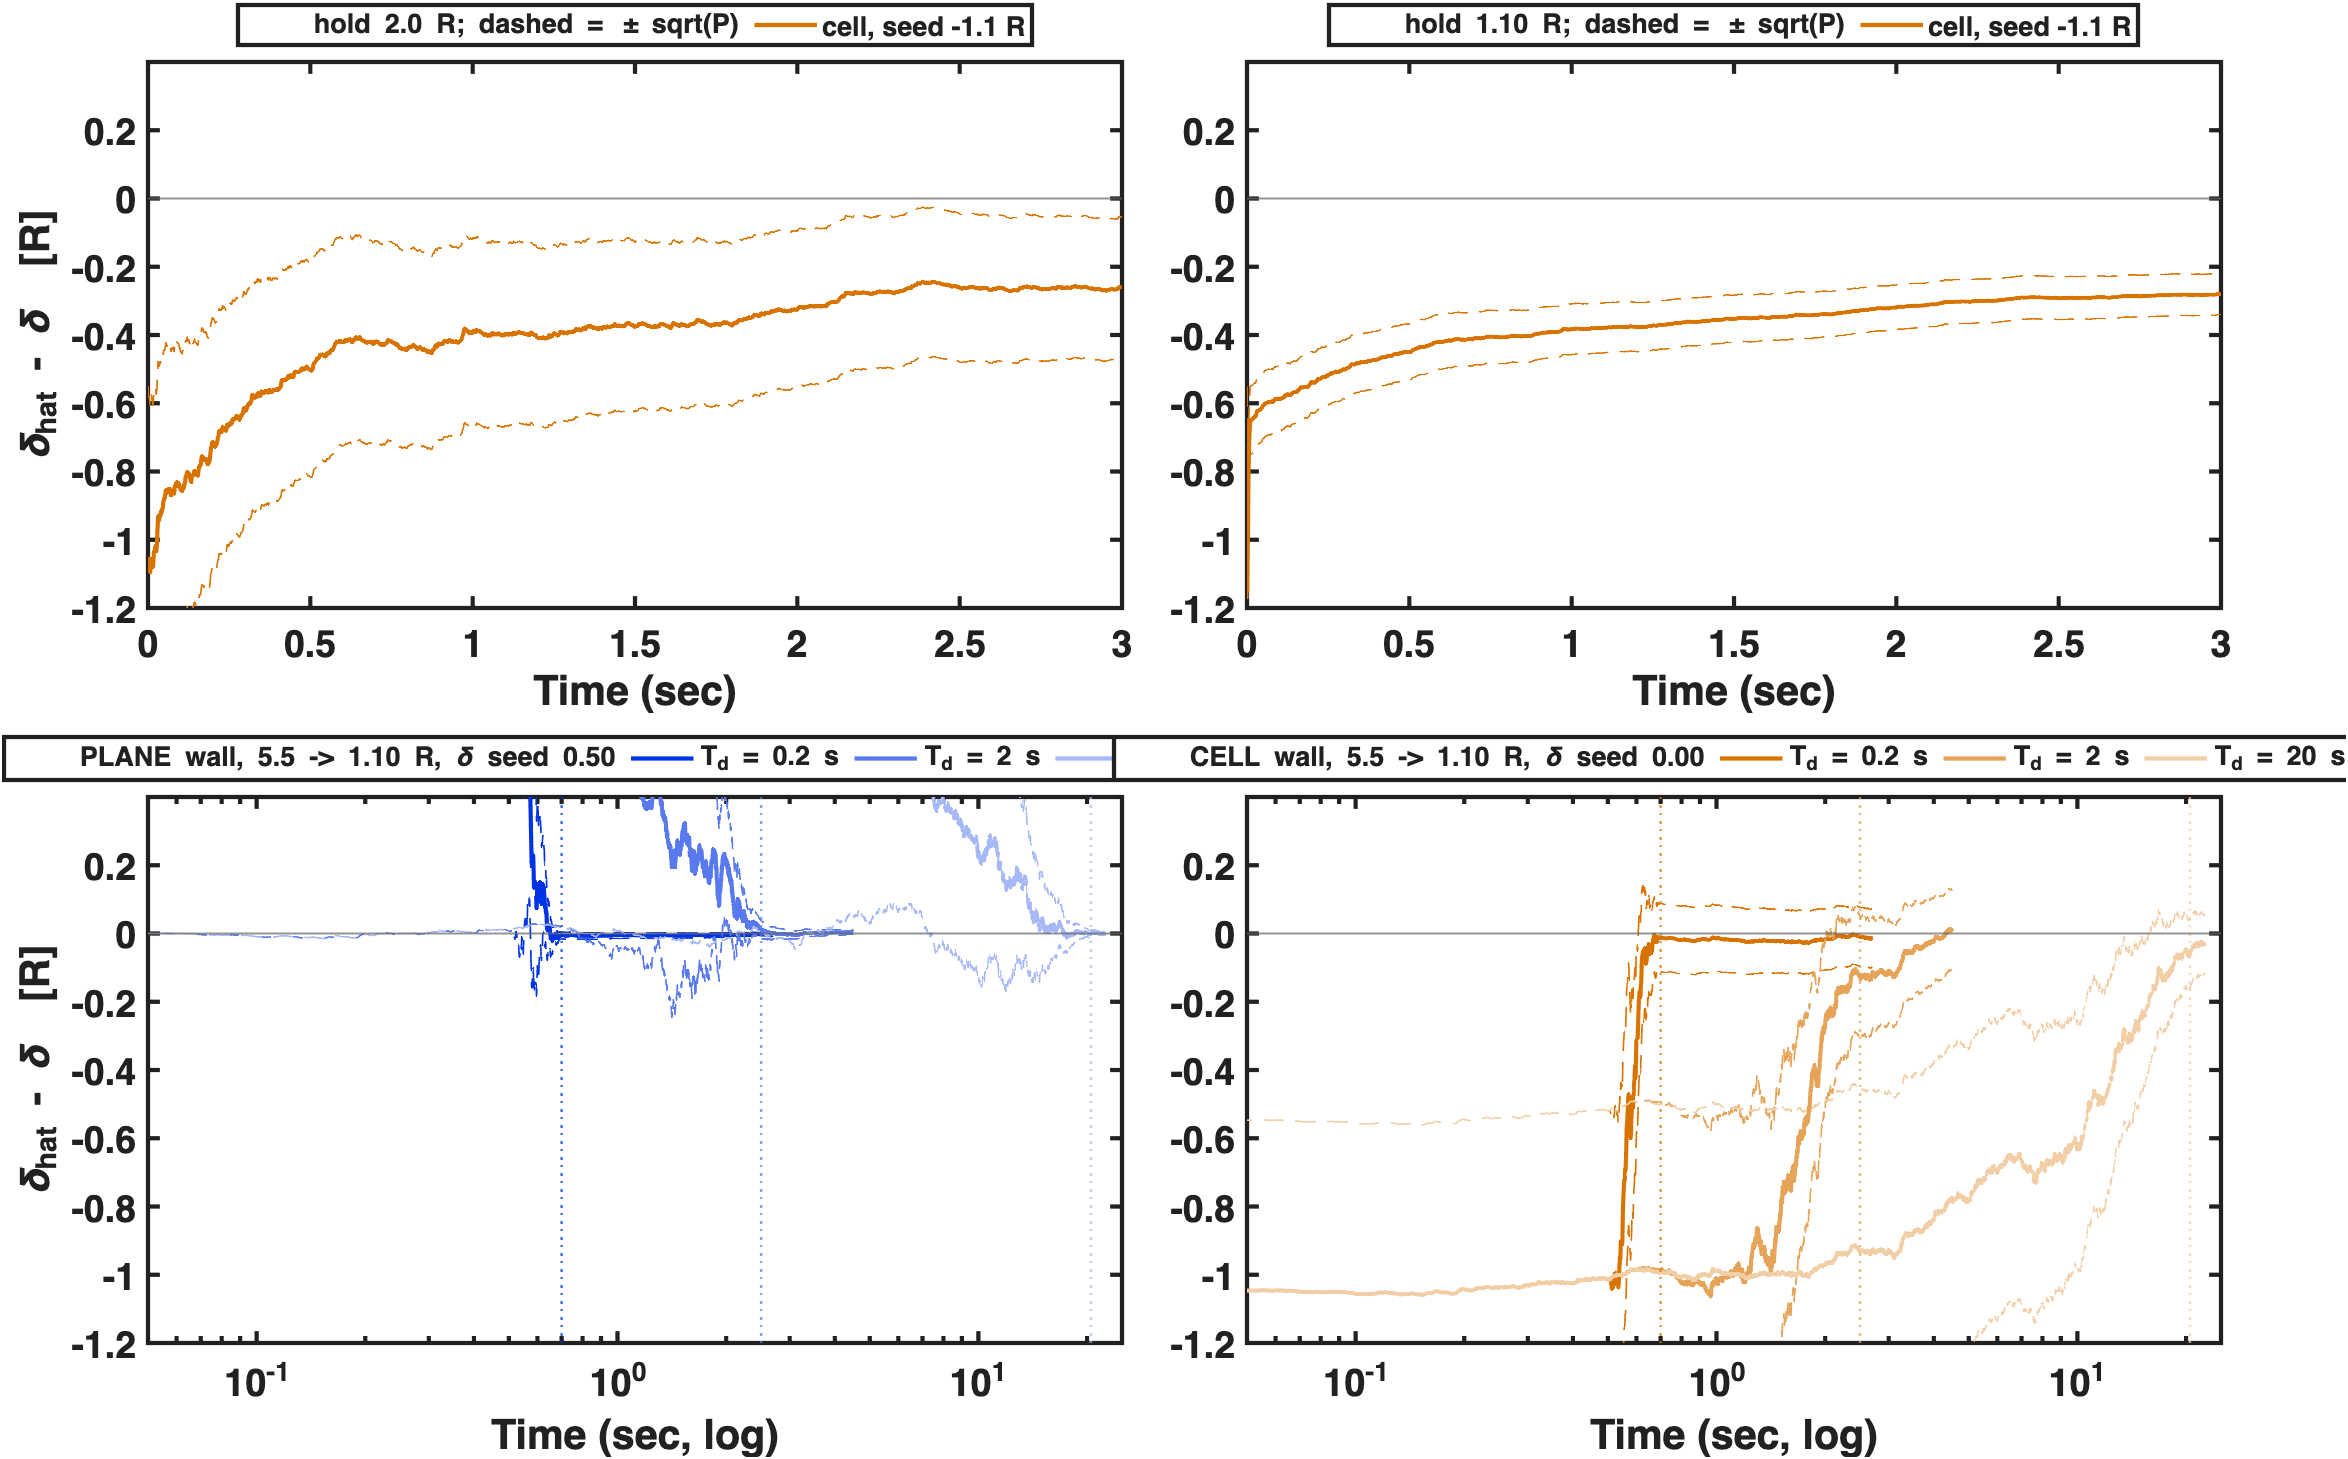
\includegraphics[width=\textwidth]{figures/delta_fixed_speed_PI.png}

\clearpage
\noindent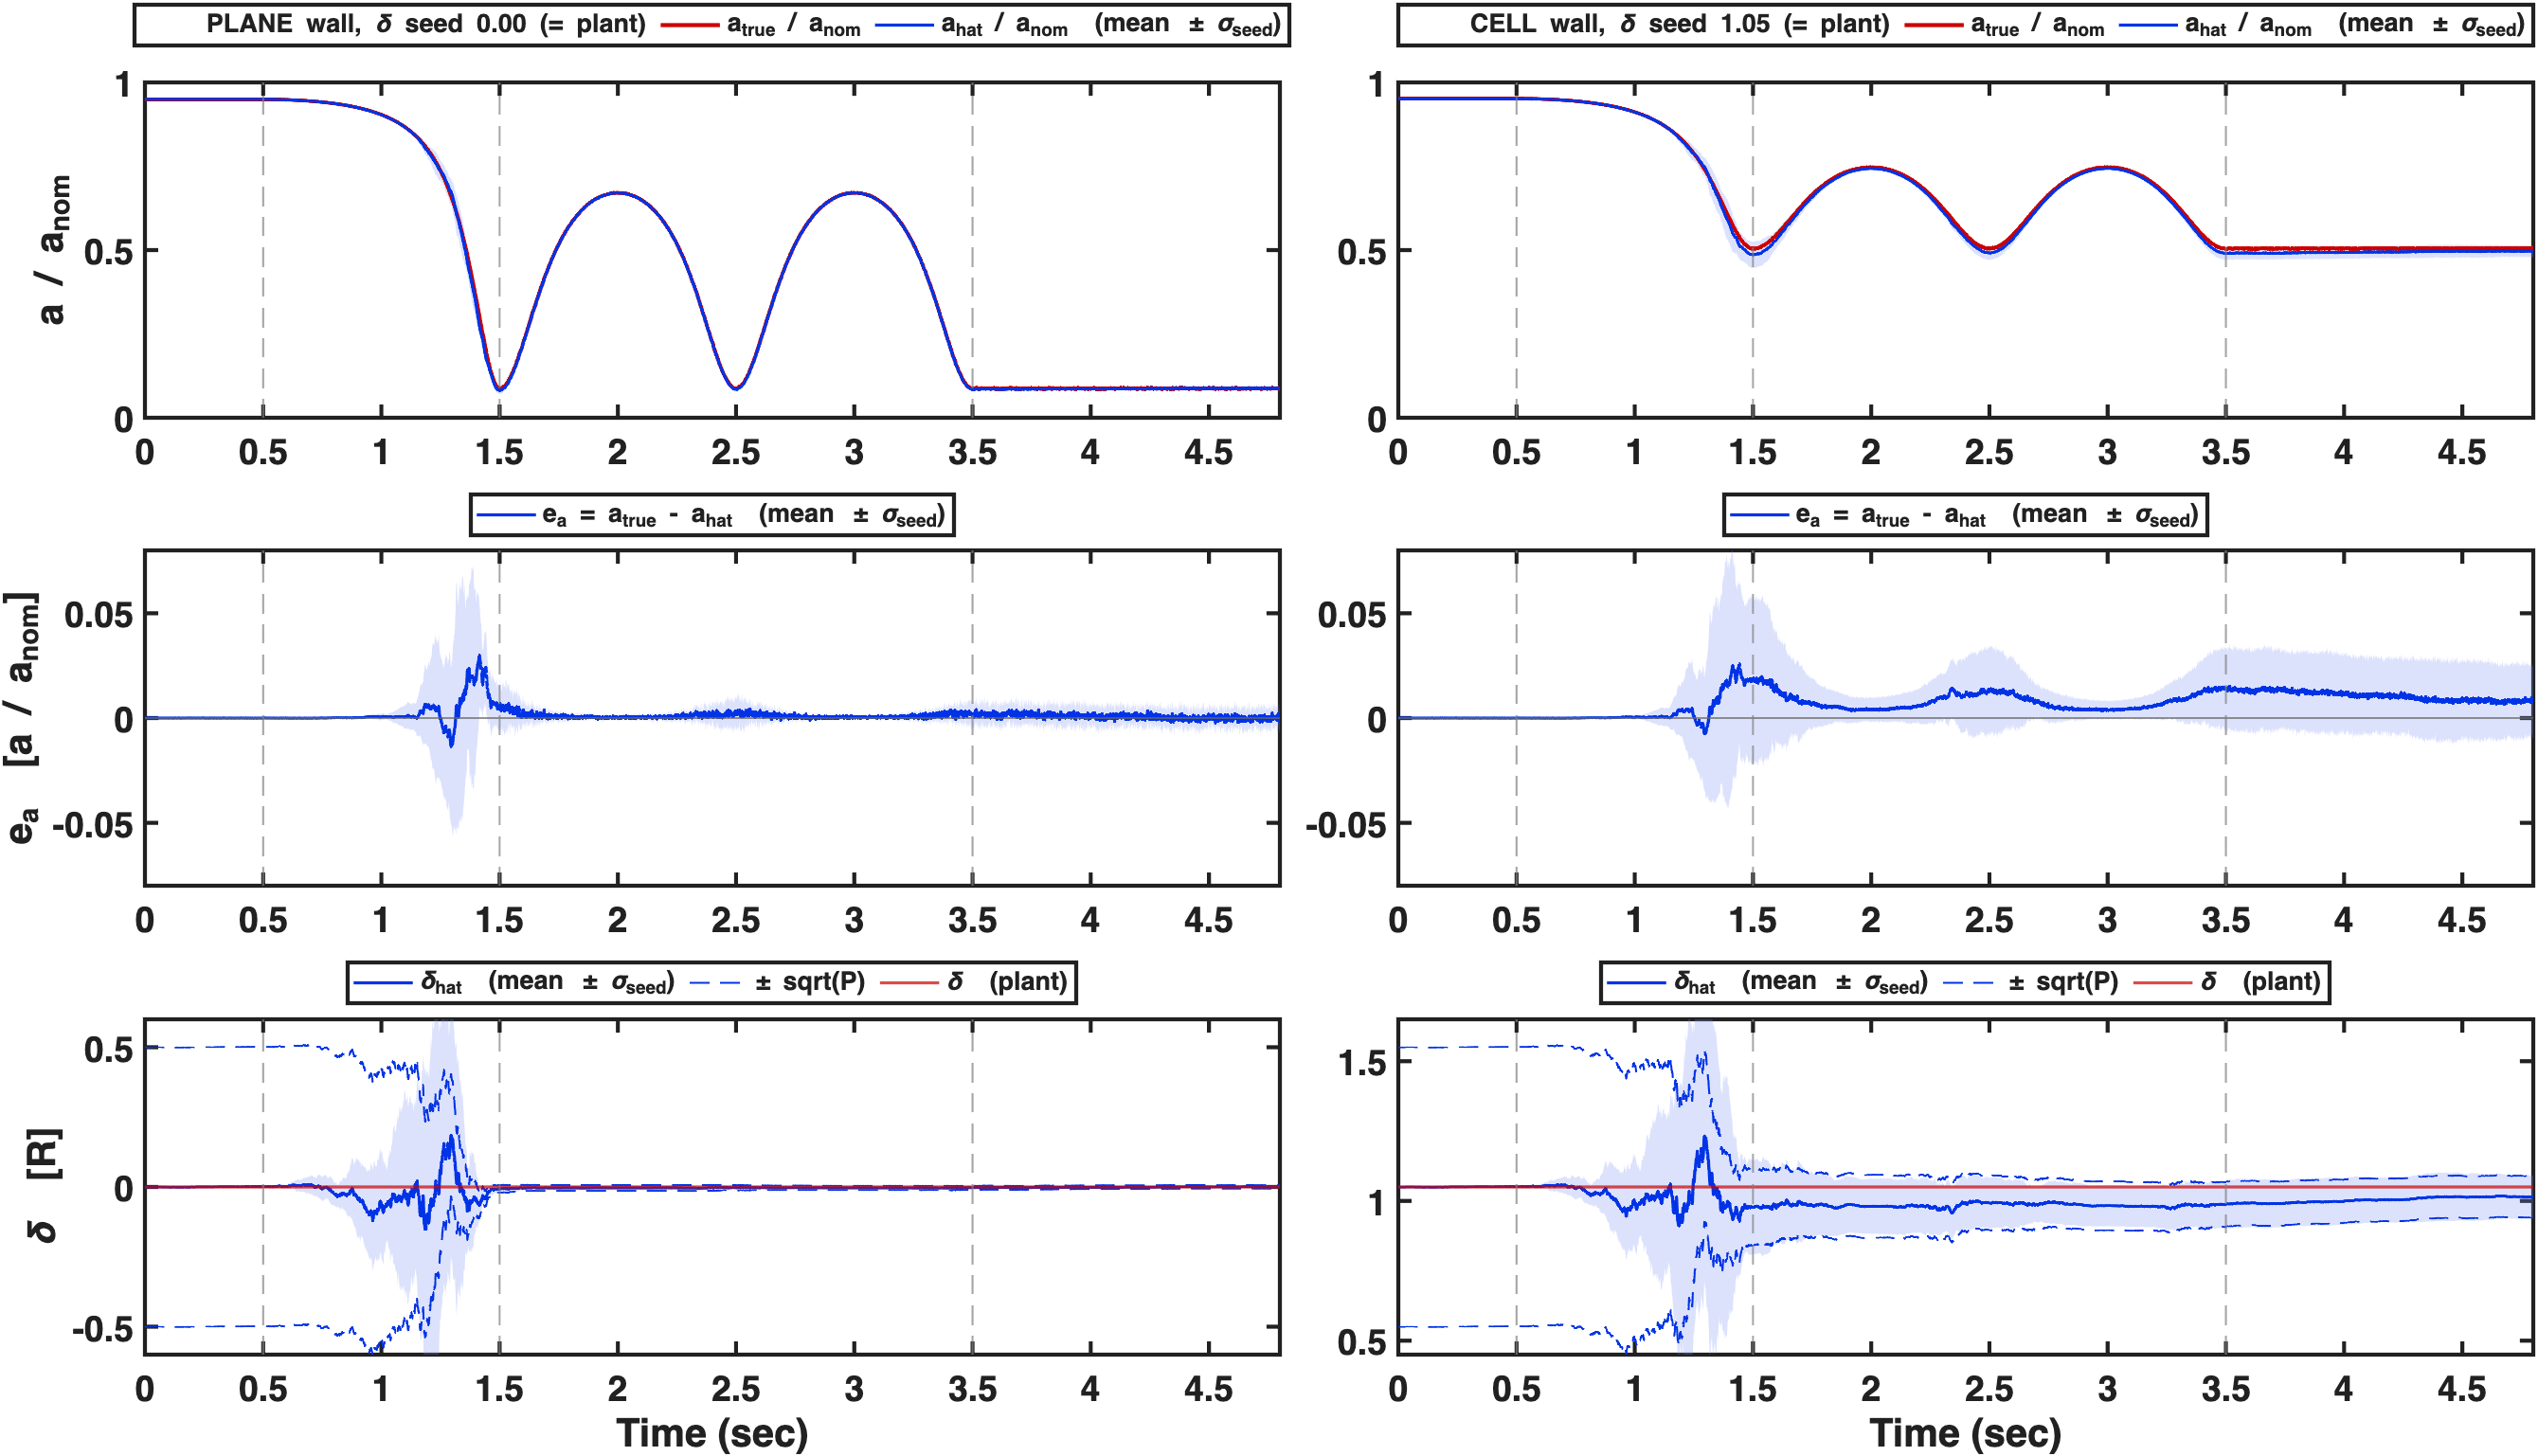
\includegraphics[width=\textwidth]{figures/ladder_delta_compact_T_plane_cell.png}

\begin{landscape}
\vspace*{\fill}
\noindent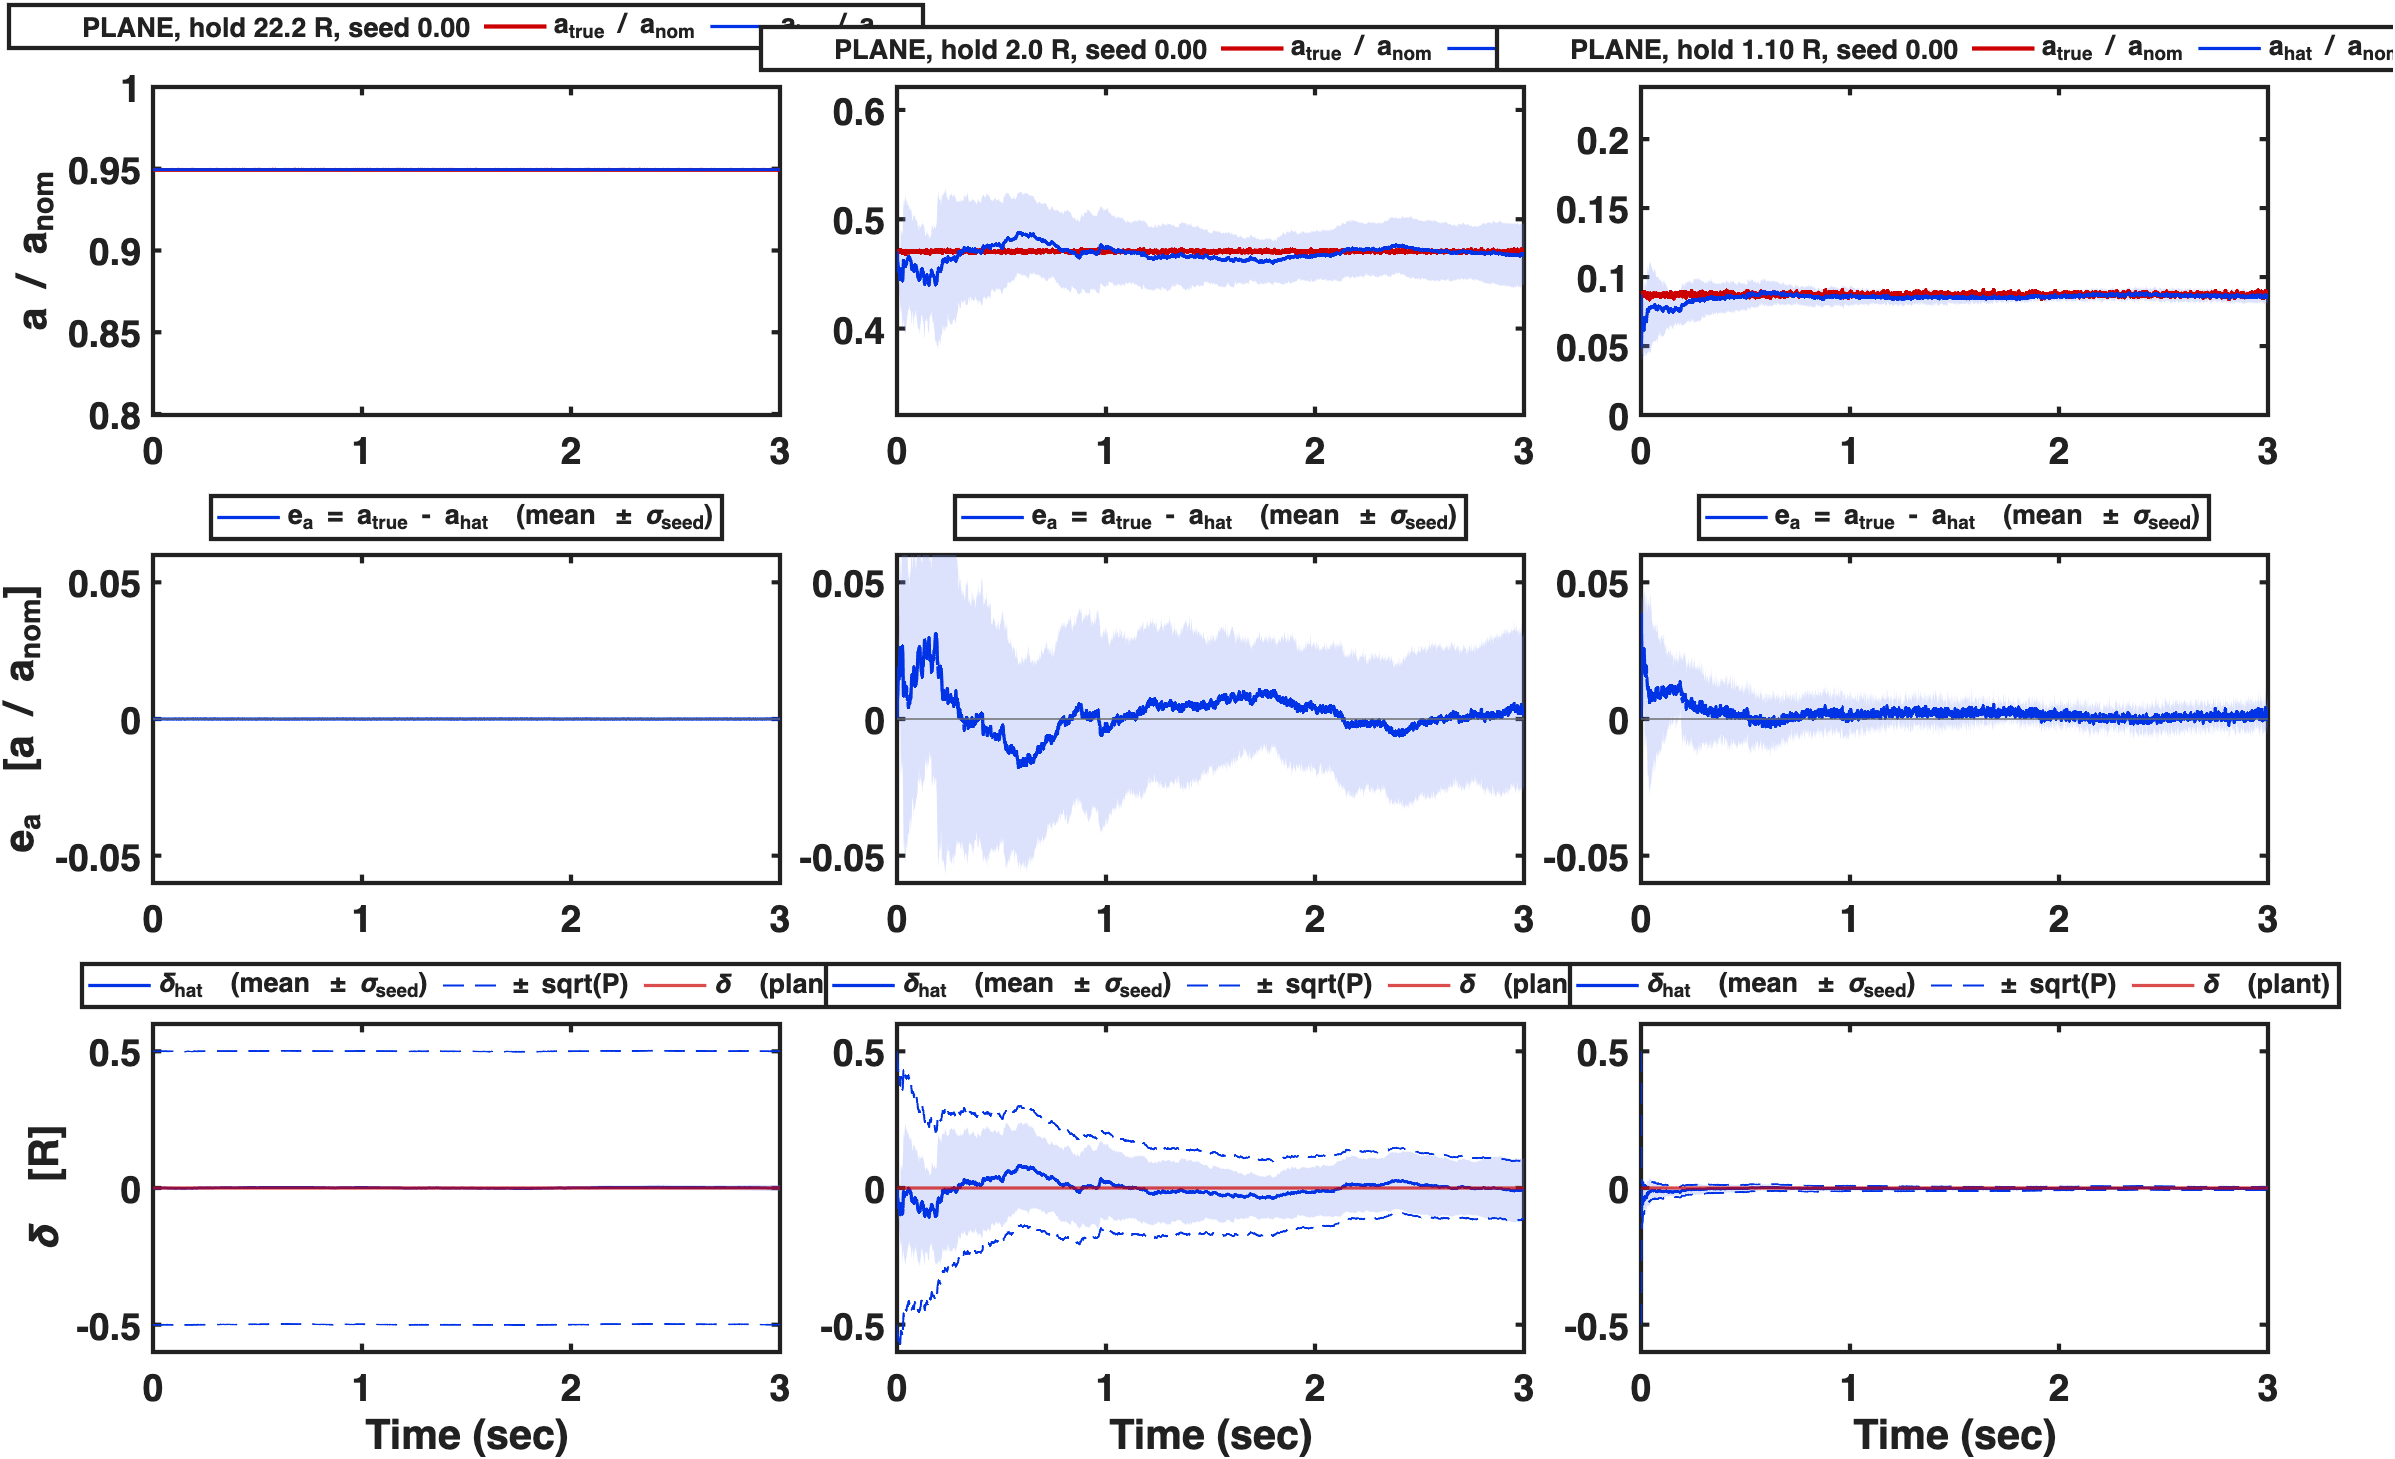
\includegraphics[width=0.93\linewidth]{figures/fixed_delta_plane_T.png}
\vspace*{\fill}
\end{landscape}

\begin{landscape}
\vspace*{\fill}
\noindent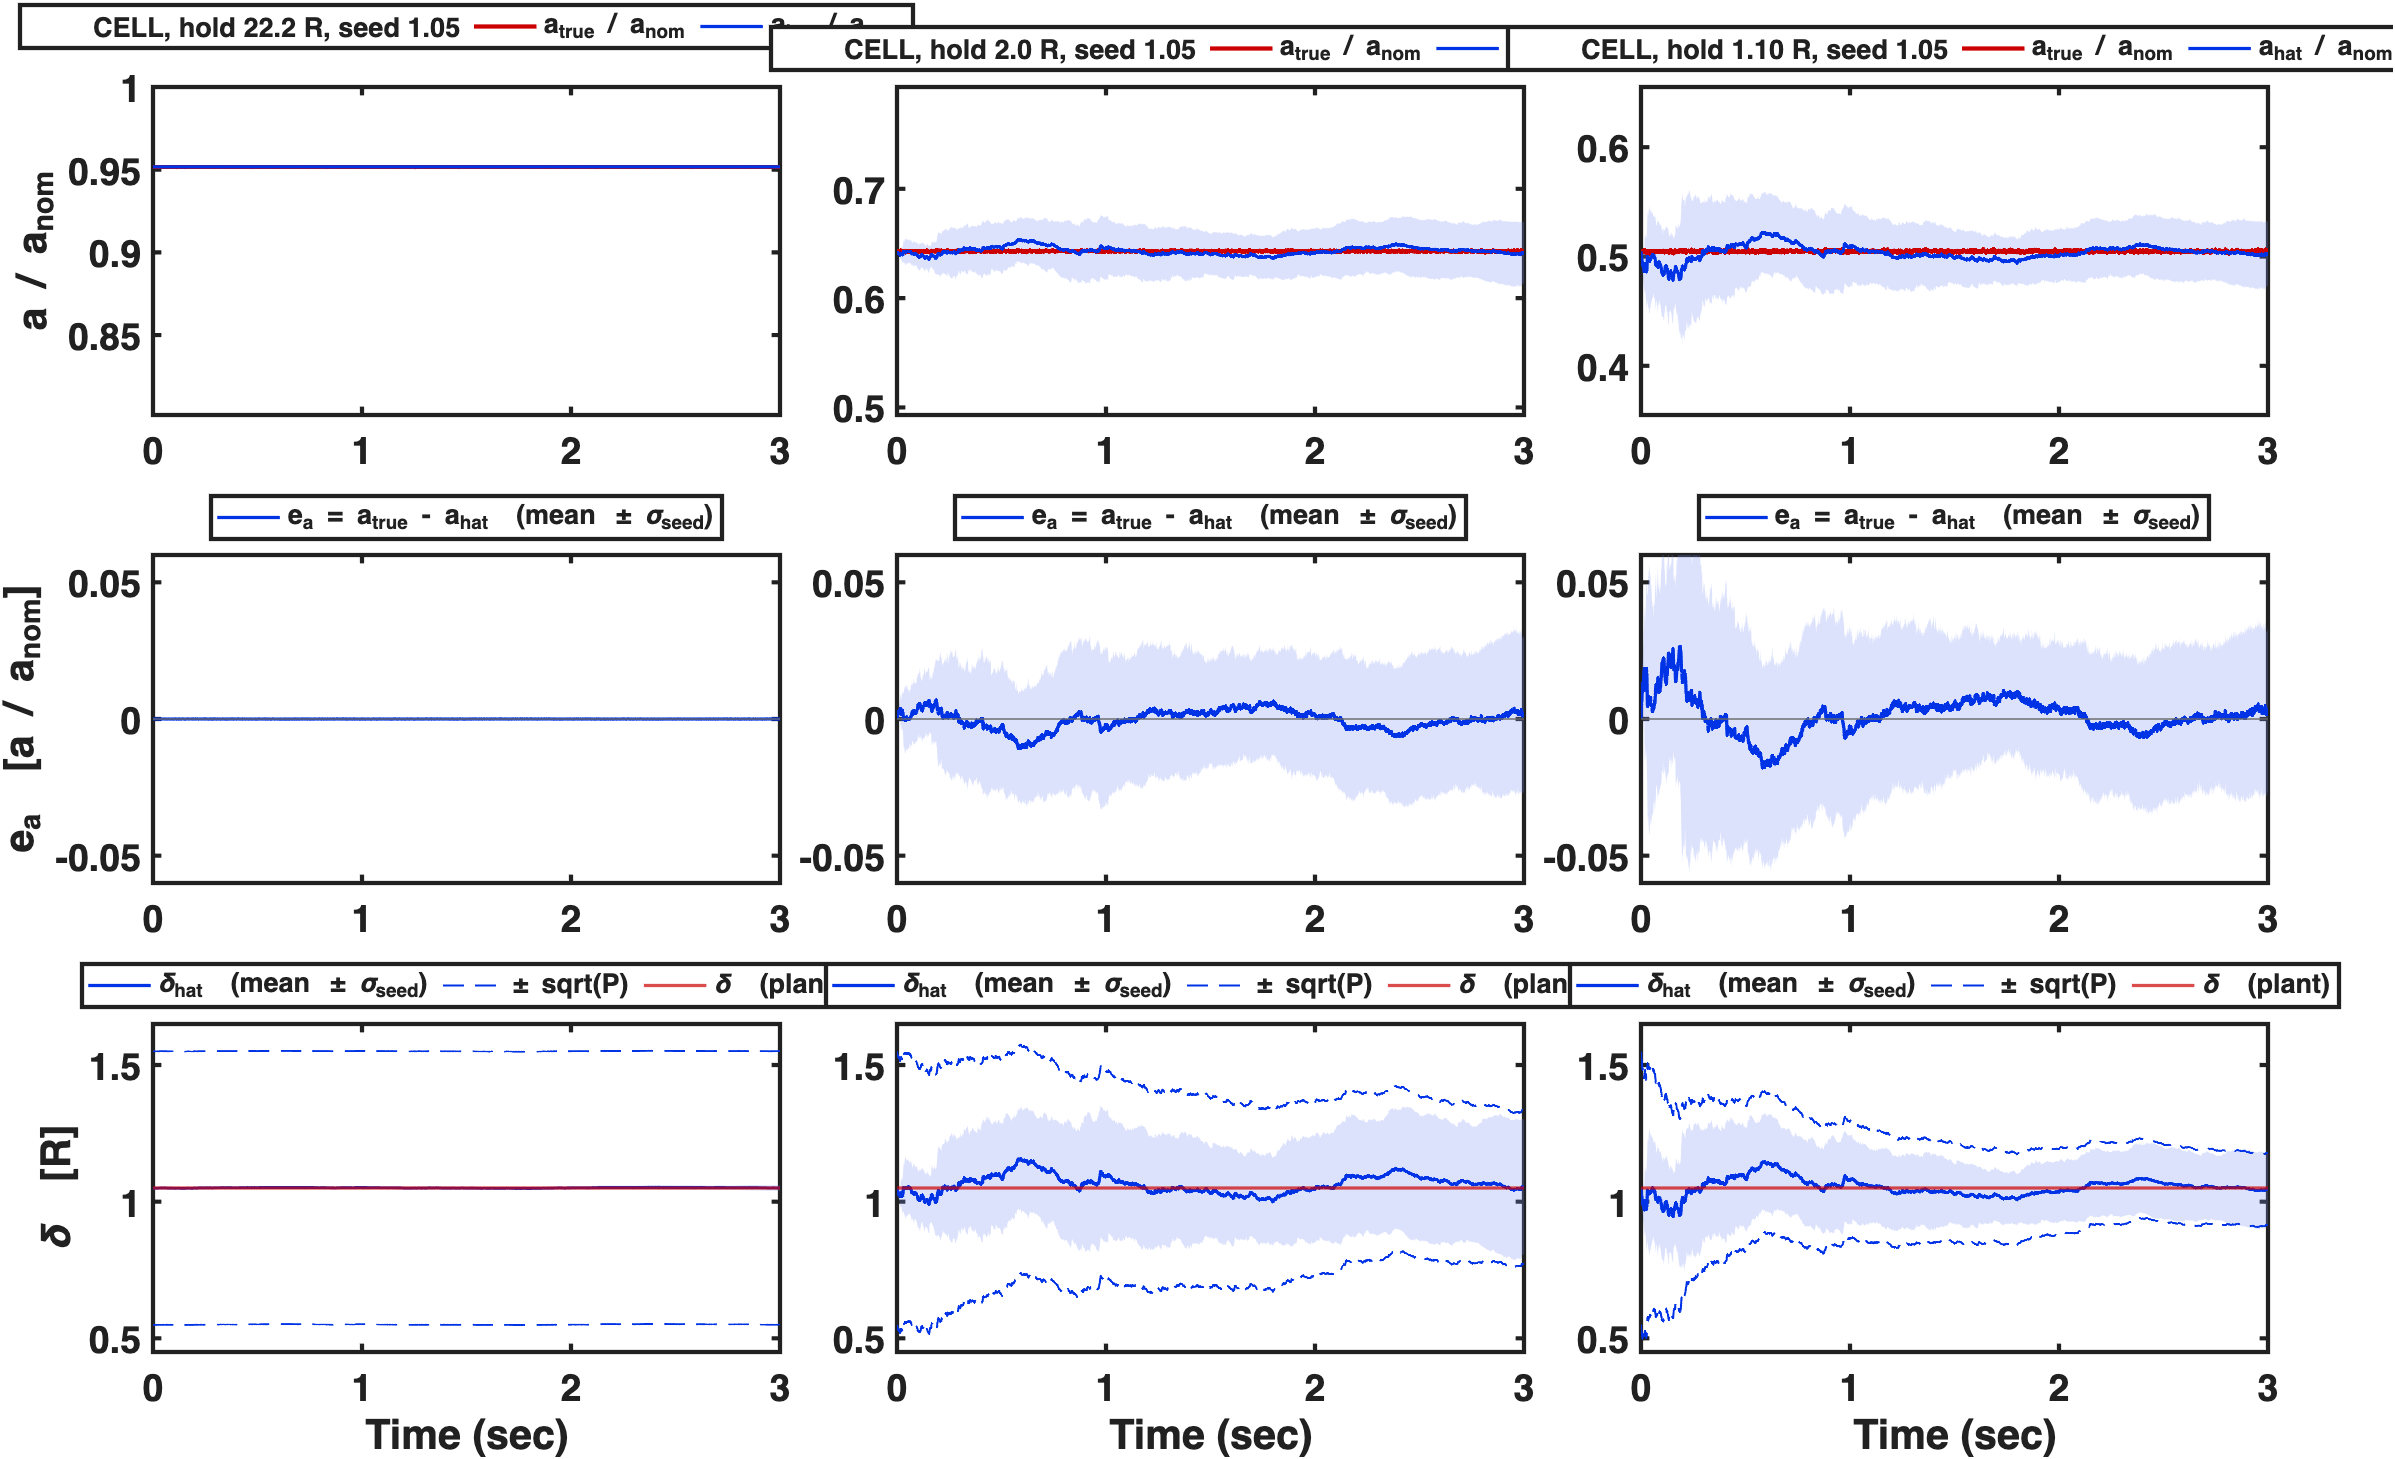
\includegraphics[width=0.93\linewidth]{figures/fixed_delta_cell_T.png}
\vspace*{\fill}
\end{landscape}

\clearpage
\noindent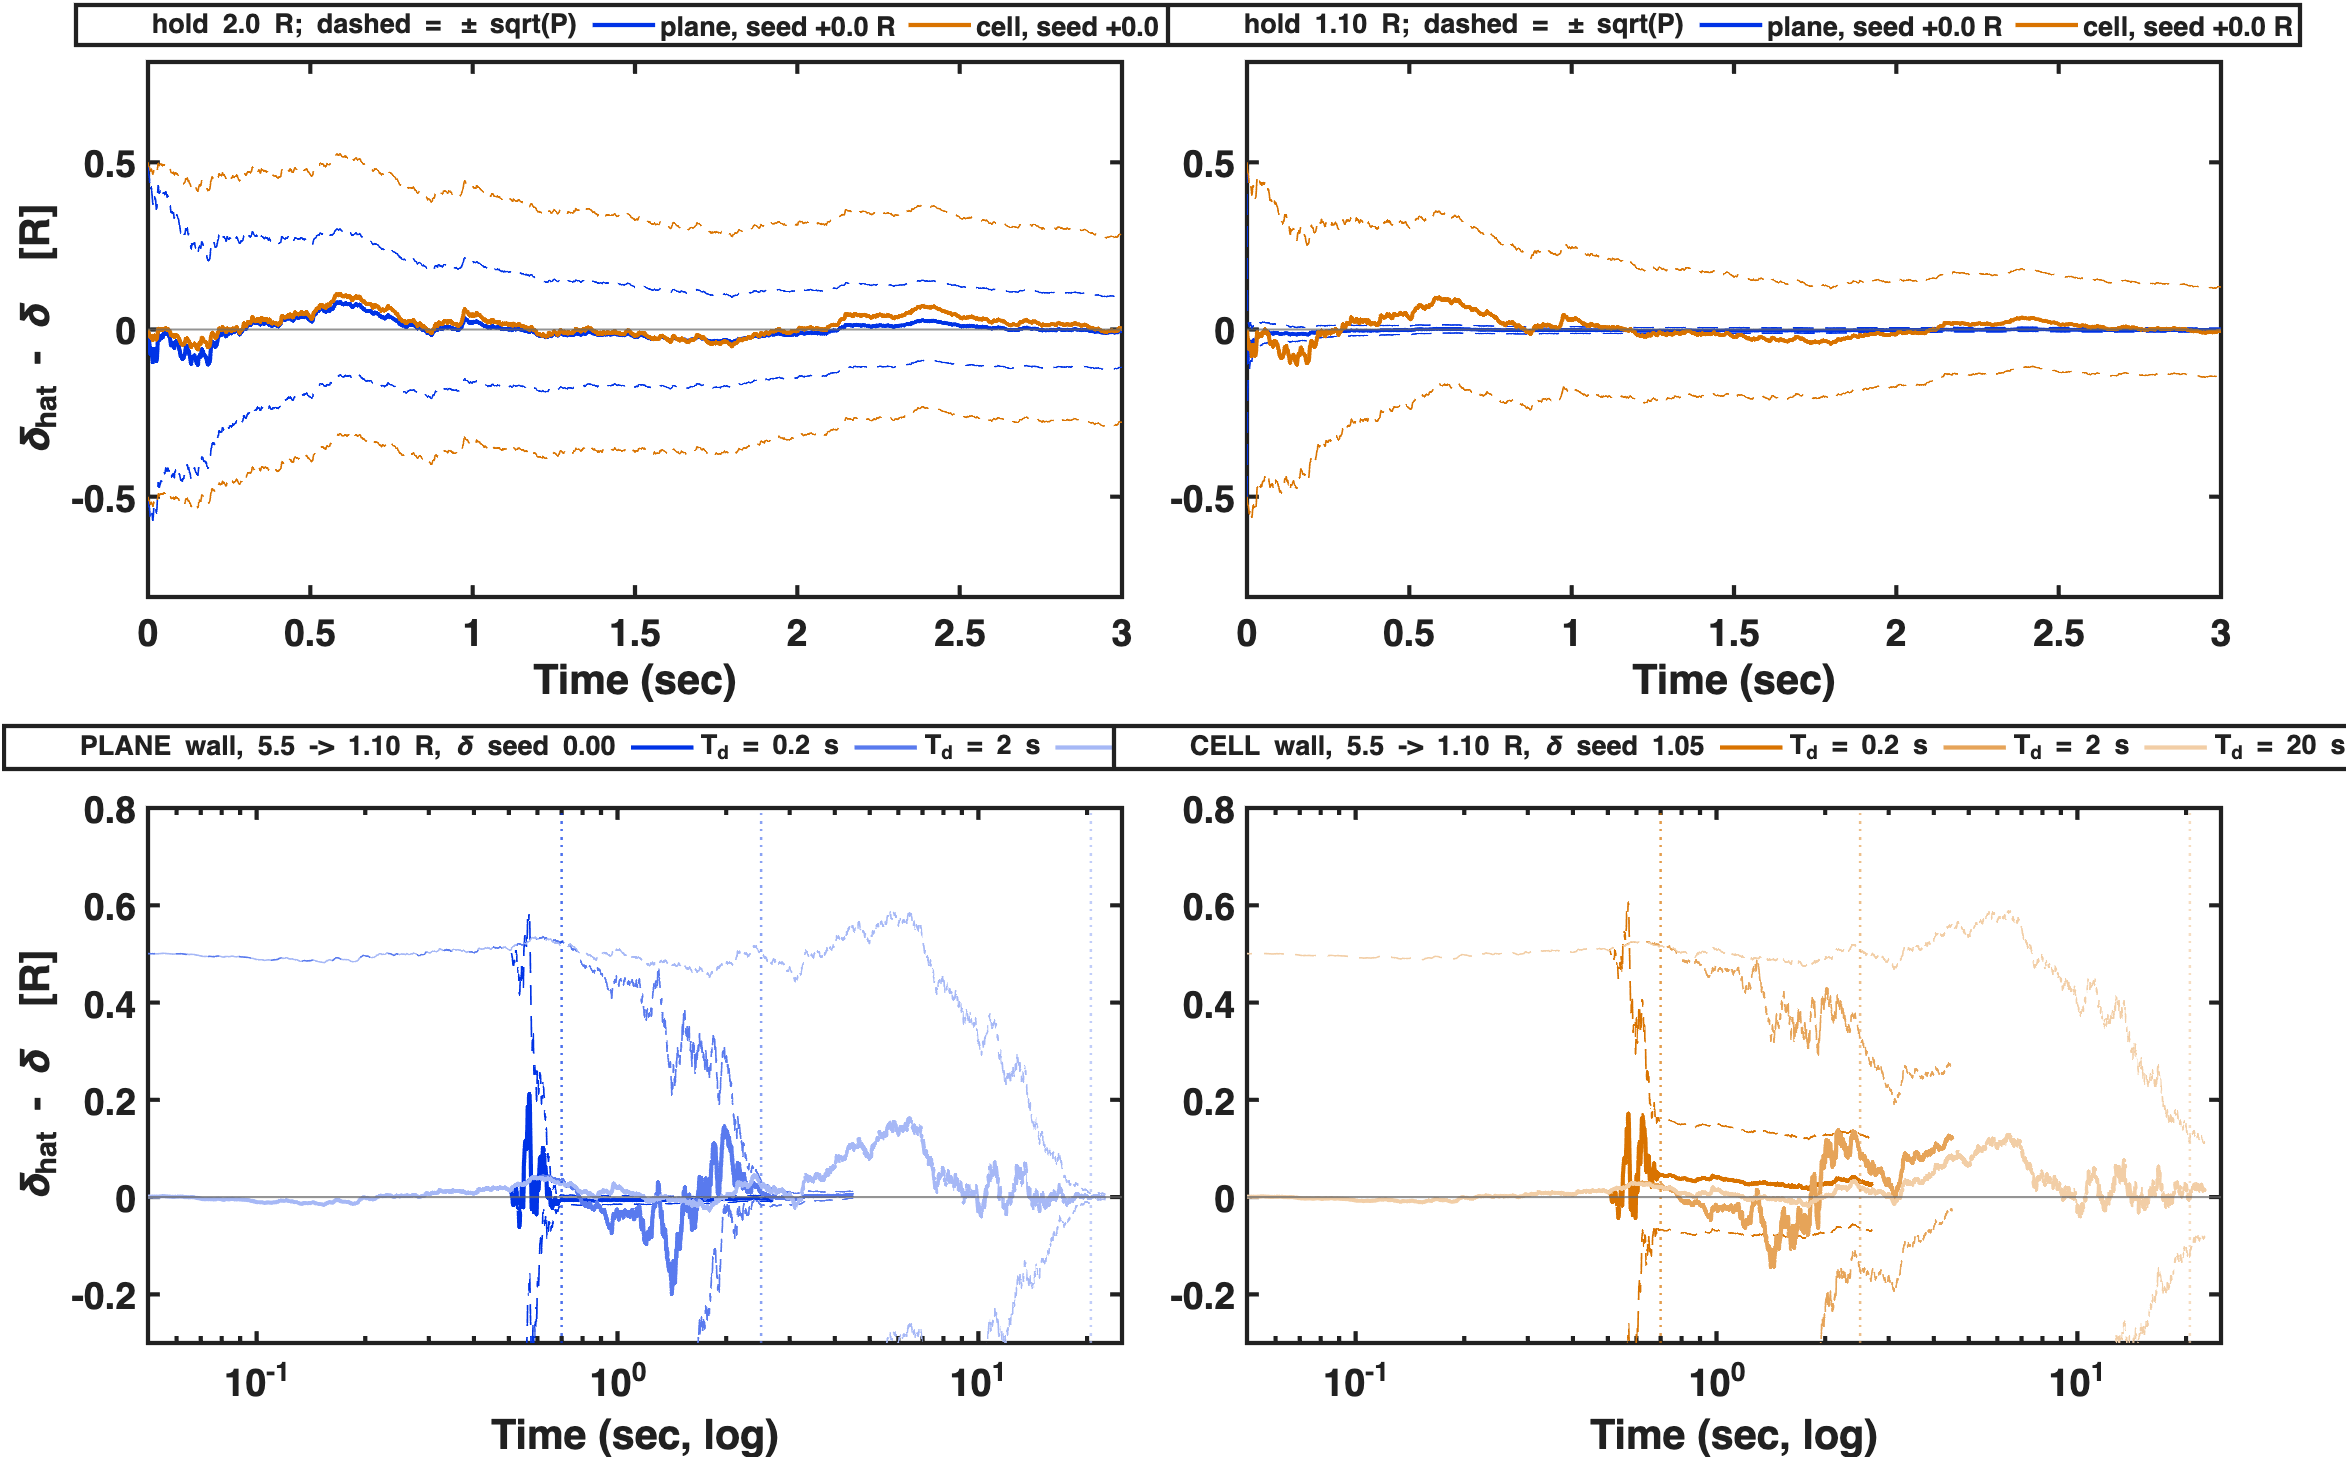
\includegraphics[width=\textwidth]{figures/delta_fixed_speed_T.png}

\end{document}
